\chapter{Optimal Dynamic Selection of Gear-ratios}  % to exploit or attenuate the external load dynamics
\label{sec:ControlAndPlanningOfRobotUsingVariableGearRatioActuators}

%\begin{flushright}
%\textit{"With four parameters I can fit an elephant, and with five I can make him wiggle his trunk."} \\ \emph{John von Neumann}
%\end{flushright}

\begin{flushright}
\textit{"He will win who knows when to fight and when not to fight."} \\ \emph{-- Sun Tzu}
\end{flushright}
\vspace{10pt}


The transmission gear-ratio that couples an actuator to a load has a significant effect upon the behavior of the actuator-load system. With a large reduction ratio, the load-side dynamics has no significant effect because it is attenuated by the factor of the square of the gear-ratio. The net load acting on the actuator is mostly its own intrinsic load, including rotor inertia and friction. In contrast, with a small reduction ratio or a direct drive system \cite{asada_direct-drive_1987}, the behavior is usually dominated by the load-side dynamics which consist of highly non-linear inertial and gravitational forces for robotics manipulators. Sometime it can be advantageous to exploit the load-side dynamics: gravity may push the robot in a desired direction; the robot may coast with small dissipative torques induced at the actuator side; or the robot joints become backdrivable to comply to an external force. In other situations, however, it may be advantageous to isolate the actuators from the load-side dynamics and external disturbances: using a large gear-ratio to bear a large load or moving it slowly against gravity, for example.

This chapter aims to explore the potentials of actuator transmissions that can be switched dynamically, such as the technology presented in chapter \ref{sec:MultipleSpeedActuationTechnology}, to either attenuate or leverage the natural dynamics of the system. Robots using lightweight VGA have the potential for achieving fast motions, high load-bearing, compliance and high-impedance, as required by diverse load conditions encountered by robotic systems. However, to truly exploit those salient features of VGA, control laws to select dynamically gear-ratios based on the current situation and task of the robot must be developed. Here in this chapter, feedback laws for robot control including gear-ratio selection are thus explored. The variable gear-ratio is used not merely for increasing maximum torque and speed, but also to significantly alter the dynamic properties, including load sensitivity, robustness, and backdrivability advantageously given the situation.

%Outline
In section \ref{sec:princ}, the principle of load leveraging and attenuation is delineated for a simple 1-DoF manipulator. Section \ref{sec:chal} will discuss related works and technical challenges. Section \ref{sec:model} will introduce a formal mathematical representation and propose a dynamic model for robotic system using VGA. Two different control approaches are explored, a model-based control synthesis in section \ref{sec:HierachicalControlApproach}, and a computational approach in section \ref{sec:DynamicProgrammingAproach}. The advantage of actively changing the gear-ratio are then illustrated with simulations in section \ref{sec:shift_sim}, and with experiments using a custom robotic arm in section \ref{sec:shift_exp}.

\subsection{Illustration of the principle for a 1-DoF manipulator}
\label{sec:princ}

Fig. \ref{fig:bigpicture} illustrates a simplified 1-DoF robotic manipulator where an electric motor is coupled to a pendulum through a gearbox with a gear-ratio $R$.

\begin{figure}[H]
 %\vspace{-10pt}
	\centering
		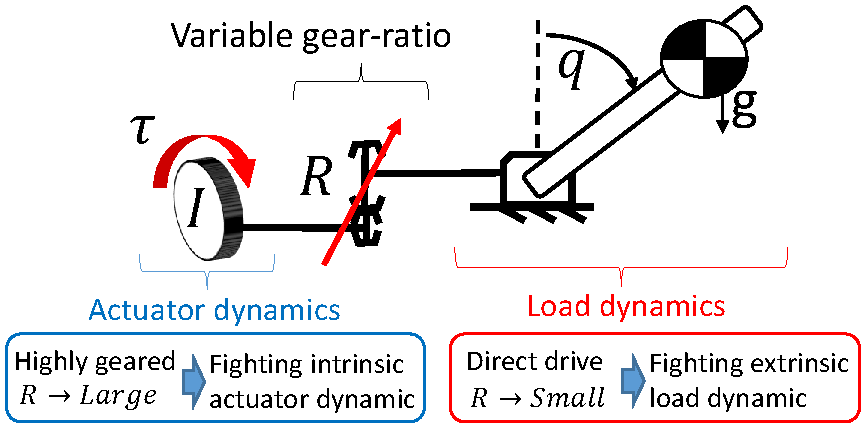
\includegraphics[width=0.75\textwidth]{gearratioeffect.pdf}
	\caption{Effect of the gear ratio on the dynamics}
	%\vspace{-10pt}
	\label{fig:bigpicture}
\end{figure}

As illustrated by phase portraits in Fig. \ref{fig:pp}, if $R$ is small then the dynamic behavior of the system is dominated by the non-linear pendulum dynamics (Fig. \ref{fig:pp1}), but if $R$ is very large, the behavior is dominated by the intrinsic inertia of the actuator, leading to the double-integrator behavior (Fig. \ref{fig:pp2}).

\begin{figure}[H]
				%\vspace{-10pt}
        \centering
				\subfloat[ Reduction ratio $R$=1 ]{ %extrinsic dynamics
				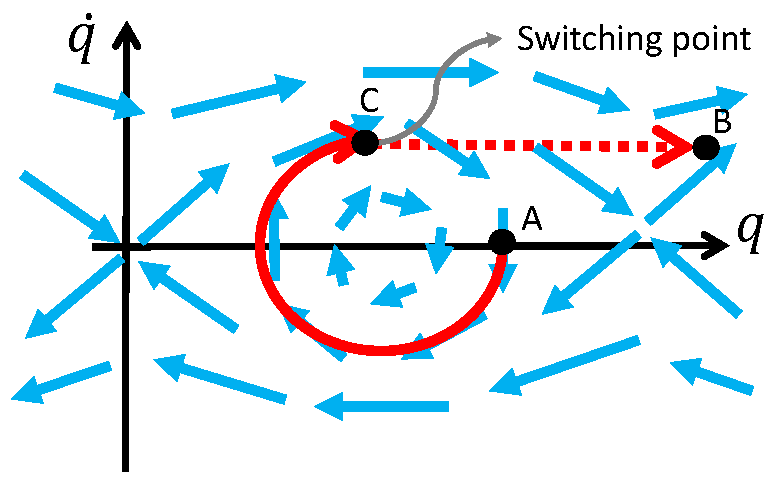
\includegraphics[width=0.40\textwidth]{pp1_hand.pdf}
				\label{fig:pp1}}
        \subfloat[Reduction ratio $R$=10 ]{ % intrinsic dynamics
				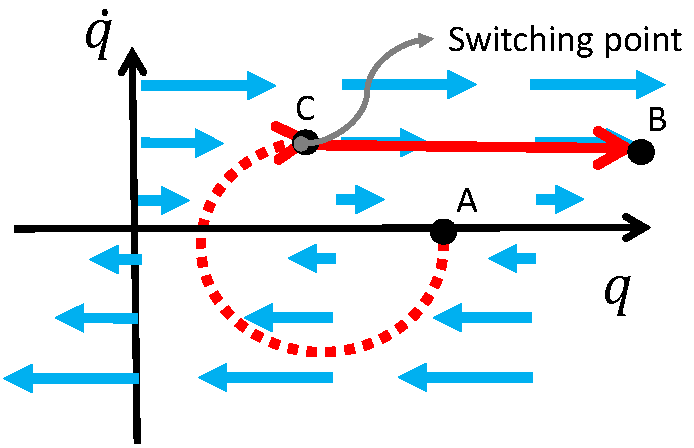
\includegraphics[width=0.40\textwidth]{pp10_hand.pdf}
				\label{fig:pp2}}
        \caption{Phase portraits illustrating the dynamical behavior}
				\label{fig:pp}
\end{figure}

The vector fields of Fig. \ref{fig:pp} illustrate the evolution of the system with no actuator torque. Suppose that we want to move from state A to state B on the phase plane. Starting off state A with the gear-ratio of 1:1 brings the system along the curved trajectory shown in Fig. \ref{fig:pp1}. Switching the gear ratio at state C to 1:10 will change the trajectory to the one in Fig. \ref{fig:pp2}, and bring the system to the destination state B. Note that no actuator torque is necessary for following this trajectory. A salient feature of actively changing the gear-ratio is that a vector field having properties useful for moving in a desired direction can be selected to minimize the necessary torque to apply to the system. 


\subsection{Challenges and related works}
\label{sec:chal}

This chapter investigates control scheme for robots equipped with variable gear-ratio actuators. While variable gear-ratio actuators have been studied extensively for automobile power-trains, they have not yet been fully investigated in robotics, despite significant potential gains. Variable gear-ratio transmissions for electric motors have been proposed for legged locomotion \cite{hirose_design_1991}, grasping robotic hands \cite{shin_robot_2012} , propulsion system \cite{lee_new_2012} \cite{mckeegan_antonovs_2011} and actuation systems \cite{girard_two-speed_2015} \cite{hirose_development_1999} \cite{tahara_high-backdrivable_2011}. Some of those works address the issue of how to change the gear-ratio, but there is no general approach to the high-level control of automatically selecting the right gear-ratio for nonlinear, coupled multi-DoF robotic systems.

From the control perspective, automating the gear-ratio selection in a robotic context is a new and challenging problem. Gear-shifting is a very non-linear process and the plant becomes a hybrid dynamical system if the usable gear-ratios are a set of discrete values. Hence most control engineering tools are not suited to tackle this problem. In simple scenarios, the gear-ratio selection can be based on simple principles. For instance, for a system running at a steady speed, the best gear-ratio can be selected based on efficiency. Alternatively, for rapid acceleration, the gear-ratio may be selected based on the actuator-load inertia matching \cite{giberti_effects_2010} \cite{chen_generalized_1991}. A robot, however, experiences diverse types of forces acting simultaneously. These include gravity, friction, and inertial forces as well as Coriolis and centrifugal forces. Hence, it is challenging to find a general control policy for selecting gear-ratios for the multitude of dynamically interacting actuators in the robotics context. 

\paragraph{Trajectory planning}

In robotic, a trajectory planning problem is usually formulated as an optimization problem. Most optimal control techniques are based on either variational approaches or some form of gradient descent to find a trajectory that minimize a cost function \cite{betts_practical_2010}. Hence those techniques cannot be used directly to optimize discrete variables. An interesting approach to get around this problem is to use the switching instants as optimization parameters instead \cite{xu_optimal_2004}\cite{majdoub_hybrid_2010}. However, to use this approach a sequence of operating modes must be predefined first. Mixed-integer programming can be used to generate optimal open-loop trajectories of dynamical system with both continuous and discrete input variables \cite{richards_spacecraft_2002}. For instance, mixed-integer programming has been used to generate optimal open-loop trajectories for a car with both a continuous torque and a discrete gear-selection input \cite{gerdts_solving_2005}. Computation time was however in the order of hours for a 6 sec trajectory. 

Sample-based planning scheme can also be used to find efficient trajectory \cite{lavalle_planning_2006}. These algorithms work generally better then optimization approaches when tackling highly-constrained system and when the goal is only to find a feasible trajectory and not necessary the optimum. The other advantage is that discrete control action can be considered without problem as these algorithm works with discretized version of the system evolution.

Open-loop trajectories can be unstable and if the system deviate from the original plan due to uncertainty, the optimized gear-ratio sequence might be completely unadapted after some time. For a robotic system to really leverage the advantage offered by multiple gear-ratios, it would be advantageous if gear-ratios are selected actively based on the actual conditions of the system. This chapter focus on finding closed-loop policy for the gear-ratios.

\paragraph{Feedback control}

One possible approach for closing the loop would be simply to re-plan trajectory continuously online. However, the rate at which this would be possible for hybrid robotic system would not be sufficient. Here we aim at having control policies that can react to a situation in a matter of milliseconds, for instance down-shifting as a robotic leg touch the ground. 

Most of the analytical results regarding feedback control of hybrid systems are for specific cases, for instance the optimal feedback law of linear hybrid systems with linear constraints for a quadratic cost function have been shown to have a particular form \cite{borrelli_dynamic_2005}. One computational technique that generate feedback laws and that can be used for non-linear systems with any kind of constraints is dynamic programming \cite{donald_e._kirk_optimal_2004}. Two disadvantages of the techniques are however that it only works for low-dimensional systems (so called curse of dimensionality) and also that the resulting feedback laws are in the form of a look-up table. This approach is investigated in section \ref{sec:DynamicProgrammingAproach}, which is an extention of work already published by the author \cite{girard_practical_2016}.

An alternative model-based approach is proposed in section \ref{sec:HierachicalControlApproach} with the advantage of scaling to high-dimensional robotics system, and easily applicable to trajectory tracking problems. The work in that section is an extension of a journal paper, but present improved algorithms \cite{girard_leveraging_2017}.



\newpage

\section{Control architecture}
\label{sec:arch}

This chapter proposed control schemes to dynamically select the optimal gear-ratios online. The focus is on feedback policies, that can react quickly to the states of the robot, and engage the appropriate gear-ratio with minimal delays (in the order of 20 ms). Two approaches are investigated and illustrated at Fig. \ref{fig:controlarchitectures}. 

\begin{figure}[H]
				%\vspace{-10pt}
        \centering
				\subfloat[ Dynamic programming approach ]{ % intrinsic dynamics
				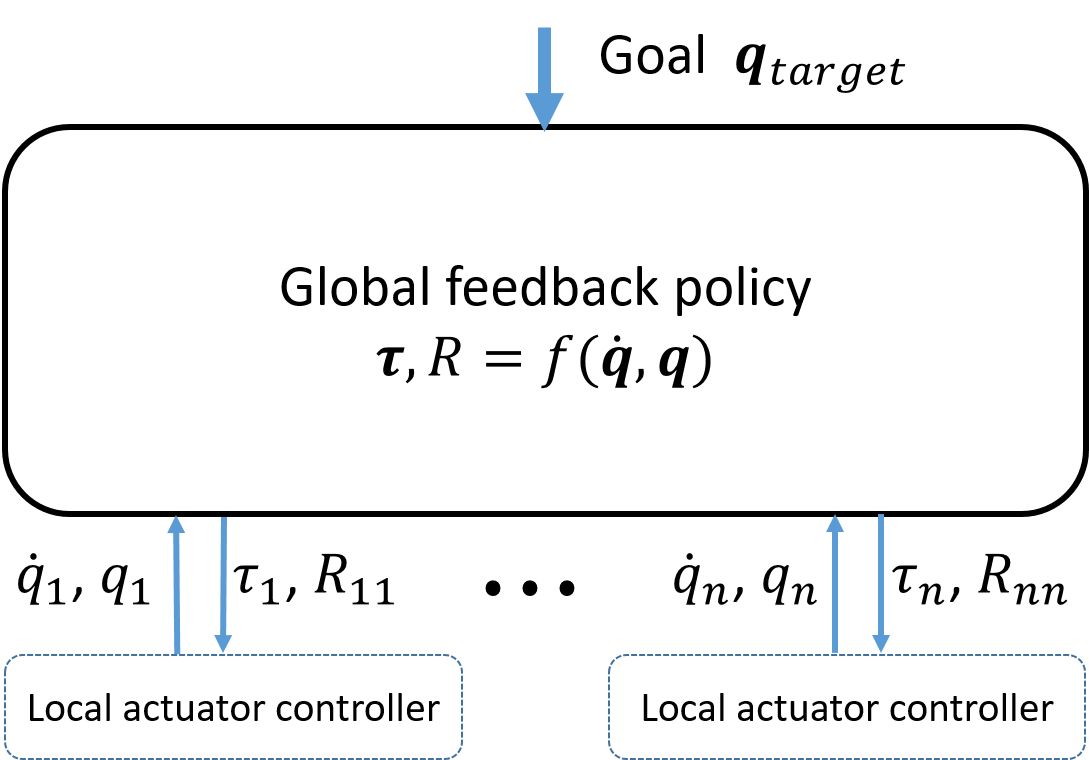
\includegraphics[width=0.45\textwidth]{archi2.png}
				\label{fig:archi2}}
				\hspace{+10pt}
				\subfloat[ Model-based approach ]{ %extrinsic dynamics
				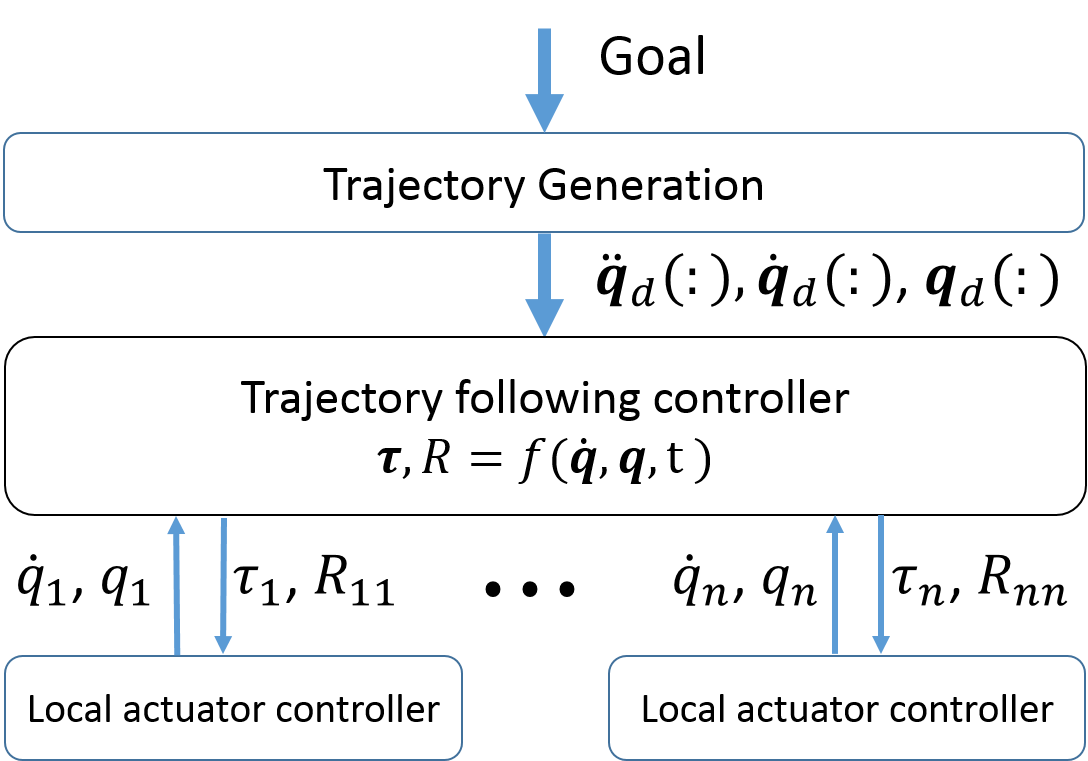
\includegraphics[width=0.45\textwidth]{archi3.png}
				\label{fig:archi3}}
        \caption{Proposed Control Architectures}
				\label{fig:controlarchitectures}
\end{figure}

The architecture of both control approaches is designed so the control signal is a torque and a gear-ratio for each actuator. Hence, it is assumed that low-level VGA controllers handle tracking the torque setpoint and the gear-shifting process. This is analogous to a situation where the robot would be a car with a semi-automatic transmission, and designing policies for the driver where the two control inputs are a throttle level a and shift-up/shift-down signal. The low-level VGA controllers would be specific to the type of actuator used in the system. For the particular case where the VGA are DSDM actuators, the low-lever controllers would be the control laws described in Chapter \ref{sec:MultipleSpeedActuationTechnology}. The architecture difference is that, for the dynamic programming approach given a goal (a target robot configuration $\vec{q}_{target}$) a feedback policy is generated directly. However, for the model-based approach the high-level controller is separated into two levels. A feedback policy for trajectory tracking and a open-loop motion planning algorithm a generate a reference trajectory to reach the goal. 

\paragraph{Trajectory Generation} Algorithm synthesizing a dynamic trajectory that meets performance requirements for reaching the target robot configuration starting at the actual robot configuration: 
%
\begin{align}
  \ddot{\vec{q}}_d(:),\dot{\vec{q}}_d(:),\vec{q}_d(:) = f_{planner}(\vec{q}_{target}, \vec{q})
	\label{eq:trajgen}
\end{align}
%
Computation time is in the order of 1-10 sec depending the robot complexity. Hence, this step is done offline in advance, or alternatively in closed-loop by re-planning continuously but at a very low rate. 

\paragraph{Low-level actuator controller} Independent actuator controllers executing low-level hardware commands in response to given torques and gear-ratio set-points. For the particular case of a DSDM actuator the controller compute 
%
\begin{align}
  M1_{pwm} , M2_{pwm} , Brake_{pwm} = f_{DSDM}(\tau_i, R_{ii})
	\label{eq:low-level-dsdm}
\end{align}
%

\paragraph{Trajectory following controller} A function that compute torques and gear-ratios as a function of the robot actual states and the time:
%
\begin{align}
  \vec{\tau}, R = f_{ctl}(\dot{\vec{q}}, \vec{q} , t)
	\label{eq:trajctl}
\end{align}
%
 The function is synthesized based on a dynamic model of the robot and a desired trajectory. This function can be executed in closed-loop at a high sampling-rate in the order of 1 kHz.

\paragraph{Global feedback policy} A function that compute torques and gear-ratios as a function of the robot actual states. Can be executed online in closed-loop at a high sampling-rate in the order of 1 kHz. However synthesis of the policy require a learning phase that require multiple hours of computation. 
%
\begin{align}
  \vec{\tau}, R = f_{ctl}(\dot{\vec{q}}, \vec{q})
	\label{eq:globctl}
\end{align}
%


%TODO incorporate this:

%The proposed control architecture, shown in Fig. XXX, consists of three hierarchical control loops. First, a trajectory generation algorithm synthesizing dynamic trajectories that meets performance requirements for reaching desired states. Second, a closed-loop trajectory following controller consisting of a feedback law computing actuator torques $\vec{\tau}$ and gear-ratios $R$ based on the measured full state of the robot. Finally at the lowest level, independent actuator controllers executing low-level hardware commands in response to given torques and gear-ratio set-points. 

%The main scope of this paper is the trajectory following controller: the design of a feedback law optimizing gear-ratios and computing torque commands in real-time. For the trajectory generation, motion planning algorithms can be applied to optimize the overall trajectory \cite{lavalle_planning_2006}.   It is assumed that they would track the desired torque/force and handle the gear-shifting process when receiving a new gear-ratio set-point. 


\newpage

\section{Modeling Variable Gear-Ratio Actuators}
\label{sec:model}

\begin{flushright}
{%\footnotesize %\small
\textit{"With four parameters I can fit an elephant, and with five \\ I can make him wiggle his trunk."}
 }
 \emph{-- John von Neumann}
\end{flushright}
\vspace{+10pt}

In this section, a simple approach is proposed for modeling robot using variable gear-ratio actuators. Variable transmission are modeled as variable transformer elements, using the bond-graph terminology. This representation allows for a clear physical understanding of the effect of gear-ratio even for non-linear $n$-DoF systems. Furthermore, this modeling approach facilitates the implementation of a real-time optimization in the proposed controller. Limitations are discussed at section \ref{sec:limitation}.

%\begin{table}[htbp]
	%\centering
		%\begin{tabular}{ c c l }
		%
        %\hline \hline
			%$H$             &  :  & External inertia matrix \\
			%$D$             &  :  & External damping matrix \\
			%$C$             &  :  & External Coriolis/Centrifugal forces matrix  \\
			%$\vec{f}_g$     &  :  & External gravitational forces vector  \\
			%$\vec{d  }$     &  :  & External disturbances forces vector  \\
			%$R$             &  :  & Gear-ratio matrix (diagonal) \\
			%$I$             &  :  & Intrinsic actuator inertia matrix (diagonal) \\
			%$B$             &  :  & Intrinsic actuator damping matrix (diagonal) \\
			%$\vec{\tau}$    &  :  & Electromagnetic motor torques  \\
			%$\vec{q}$       &  :  & Joint coordinates position vector  \\
			%$\vec{w}$       &  :  & Actuator coordinates velocity vector  \\
			%$J$             &  :  & task-space coordinates / joint coordinates jacobian matrix\\
			%%&\text{Secondary variables:  \\
			%$\vec{f}$       &  :  & Net transmitted forces (joint coordinates) \\
			%$\vec{\tau}'$   &  :  & Net transmitted forces (actuators coordinates) \\
			%$\vec{\tau}_I$  &  :  & Sum of intrinsic forces  \\
			%$\vec{\tau}_E$  &  :  & Sum of extrinsic forces  \\
		%\hline \hline
        %\end{tabular}		
        %\caption{Nomenclature}	% Table caption must be placed on top of the table %
	%\label{tab:nom}
%\end{table}

\subsection{1-DoF system}
\label{sec:1DOFSystem}

First, a generic 1-DoF robot with a variable transmission is considered for simplicity. If the actuator's intrinsic resistive forces $\tau_I$ are approximated to a linear quantity, the equations of motion (EoM) can be written as:
%
\begin{align}
  H \ddot{q} + D \dot{q} + g( q )	&= R  \left[ \tau - I \dot{w} - B w	\right] \\
	\underbrace{\left[	H \ddot{q} + D \dot{q} + g( q )	\right]}_{\tau_{E}(\ddot{q},\dot{q},q)}
	&= R \tau - R^2
	\underbrace{\left[ I \ddot{q} + B \dot{q}	\right]}_{\tau_{I}(\ddot{q},\dot{q})} \\
	\tau &= 	\frac{\tau_{E}(\ddot{q},\dot{q},q)}{R} + R \; \tau_{I}(\ddot{q},\dot{q})
	\label{eq:1dofEoM}
\end{align}
%
where the effect of the gear ratio can be seen clearly; increasing $R$ attenuates the external dynamic terms $\tau_{E}$ but amplify the intrinsic actuator losses $\tau_{I}$ for a given trajectory.
%
Variable gear-ratios can be modeled as variable transformer elements, using the bond-graph terminology. Fig. \ref{fig:bondgraph1} shows a bond-graph representation of the model.
\begin{figure}[htp]
	\centering
		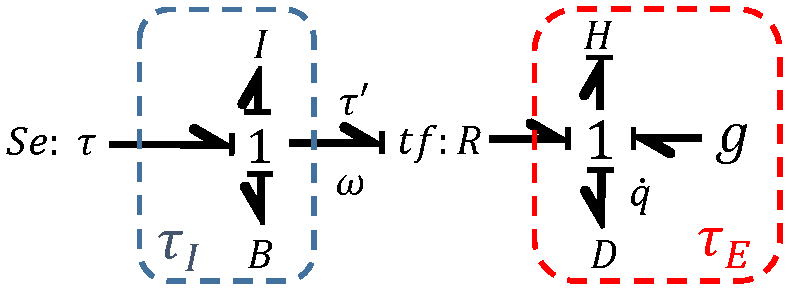
\includegraphics[width=0.70\textwidth]{bondgraph1.pdf}
	\caption{Model of a 1-DoF robot with a variable gear-ratio actuator}
	\label{fig:bondgraph1}
\end{figure}


\subsection{Generalization to $\boldsymbol{n}$-DoF manipulators}
\label{sec:GeneralizationToNDOFManipulators}

To generalize the above model to a $n$-DoF system with $n$ actuators, the load-side dynamics is considered as a generic form of manipulator equations where each port is connected to an independent actuator through a network of transformers. The network of transformers can be view as a type of coordinate transformation relating effort (force or torque) and flow (velocity or angular velocity) on the load side ($\vec{f}$,$\dot{\vec{q}}$) to those on the actuator output side ($\vec{\tau}'$,$\vec{w}$):
%
\begin{align}
	\vec{ f } = R^T \vec{\tau}' \quad  \quad R \dot{ \vec{q} } = \vec{w}
 \label{eq:coortransform}
\end{align}
%
where $R$ is a $n$ by $n$ matrix consisting of all the transformer ratios. 
%
\begin{figure}[htp]
	\centering
		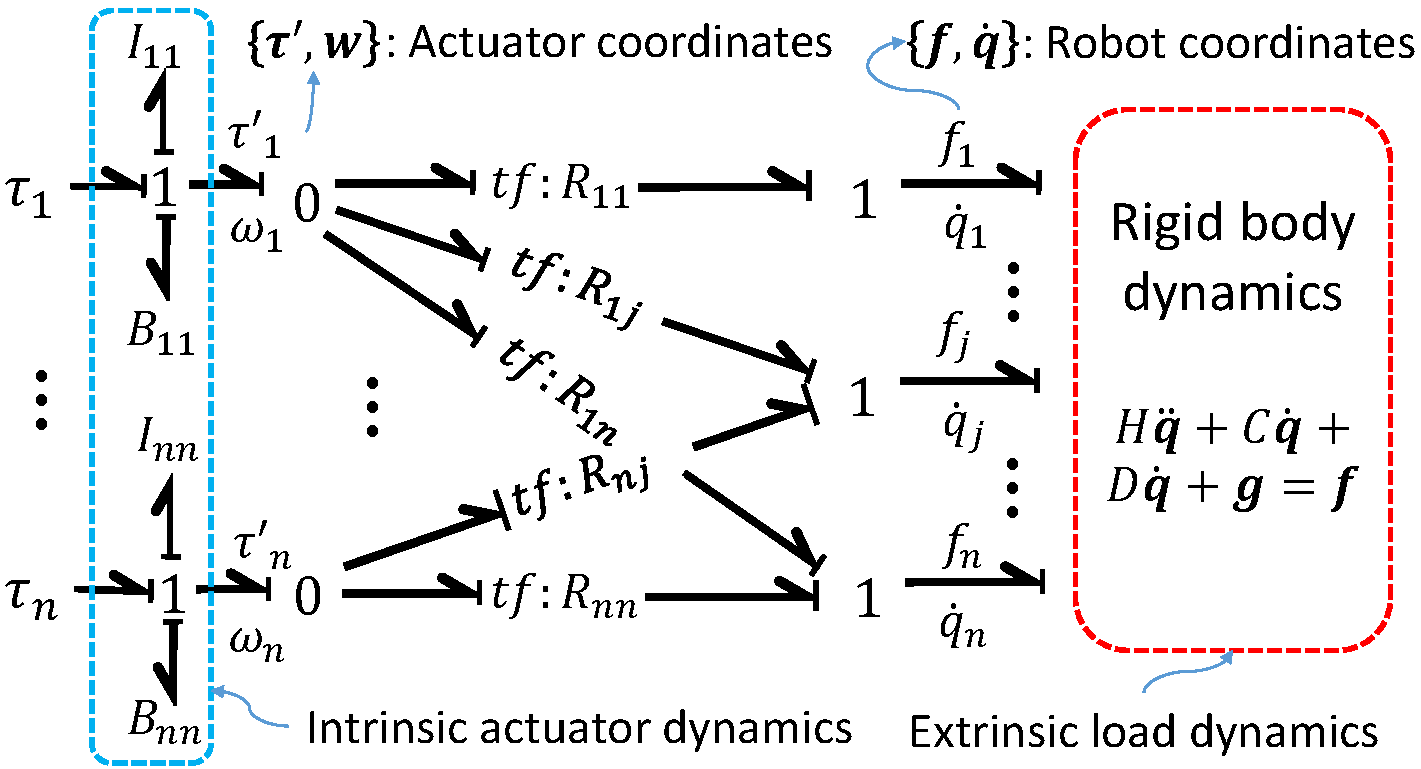
\includegraphics[width=0.80\textwidth]{bondgraph.pdf}
	%\vspace{-10pt}
	\caption{Model of a $n$-Dof robot with variable actuator-joint coupling}
	\label{fig:bondgraph}
\end{figure}

The EoM are then given by:
%
\begin{align}
	&\underbrace{ H \vec{ \ddot{q} } + C\vec{ \dot{q} } + D \vec{ \dot{q} } + \vec{ g } }_{ \vec{\tau}_{E}(\ddot{\vec{q}},\dot{\vec{q}},\vec{q})}
		= R^T \underbrace{  \left[ 
		\vec{ \tau } - I \vec{ \dot{w} } - B \vec{ w }       
		\right]}_{ \vec{\tau}' } 
 \label{eq:eom_ndof}
\end{align}
%
Note that, in the case of locomotion or manipulation where the robot interacts with the environment by physically contacting it, the dynamic model $\vec{\tau}_{E}$ must reflect the contact conditions, either by computing contact forces using constraint equations or by formulating $\vec{\tau}_{E}$ as a hybrid dynamical system.

In most practical cases, each actuator has its independent variable transmission and, thereby, the $R$ matrix will be diagonal and each diagonal value can be selected independently. Assuming this situation, the EoM can be simplified to a form, similar to the scalar case, illustrating the effect of the gear ratios matrix $R$: 
%
\begin{align}
	\vec{\tau} &= R^{-1} 
	\underbrace{ 
	\vec{\tau}_{E}(\ddot{\vec{q}},\dot{\vec{q}},\vec{q}) 
	}_{\text{External load dynamics}}
	+ R 
	\underbrace{ 
	\vec{\tau}_{I}(\ddot{\vec{q}},\dot{\vec{q}})
		}_{\text{Intrinsic losses}}
	\\ %&\text{where} \;
	\vec{\tau}_{I} &\triangleq I \vec{ \ddot{q} } + B \vec{ \dot{q} } 
	%[ \vec{\tau}_{I} ]_j &\triangleq [I]_{jj} [\vec{ \ddot{q} }]_j + [B]_{jj}  [ \vec{ \dot{q} }]_j  \quad \forall j \in {1,2,...,n}
 \label{eq:eom_ndof2}
\end{align}
%
The derivation of this simplified form is available in the Appendix \ref{sec:Rdiagndof}.

\subsection{Limitation of the simplified model}
\label{sec:limitation}
%
The main assumption of the proposed model is that gear-ratios are considered as independent control inputs, neglecting all the dynamics and delays associated with the transition of gear-ratios. Physically this implies that the kinetic energy of the system may be discontinuous at a gear-shift since the energy necessary for the transition is not considered. In the case of a car transmission for instance, this model would not keep track of the energy used for accelerating or braking the engine during the synchronization process. This model can be used if the gear-shift process is fast compared to the dynamics of the robots and if the energetic losses due to the gear-shift are negligibly small. In addition this model also assumes that all motor rotors are in an inertial reference frame, neglecting gyroscopic effects, which may be induced when the axes of motor rotors are rotated.

\subsection{Uncertainty}
\label{sec:uncertainty}

Two observations are made regarding the effect of the gear-ratios on disturbances. First, considering modeling errors and external forces on the extrinsic side as unknown generalized forces $\vec{d}$, the EoM given by eq. \eqref{eq:eom_ndof2} becomes:
\begin{align}
	\vec{\tau} &= R^{-1} 
	\vec{\tau}_{E}(\ddot{\vec{q}},\dot{\vec{q}},\vec{q}) 
	+ R 
	\vec{\tau}_{I}(\ddot{\vec{q}},\dot{\vec{q}})
    + R^{-1}
    \underbrace{ 
	\vec{d}
	}_{\text{Disturbances}}    
 \label{eq:eom_ndof3}
\end{align}
where it is assumed that the actuators are accurately modeled. Note that the effect of the disturbances is inversely proportional to the gear-ratios, and thereby attenuated when using large gear-ratios. 

Second, large gear-ratios also decrease the sensitivity of the system to uncertainty. The error of computed accelerations will be attenuated with large gear-ratios because of the larger  actuator inertia reflected to the extrinsic side:
\begin{align}
	\vec{\ddot{q}}_e &= \vec{\ddot{q}} - \vec{\ddot{q}}_r = 
	\left[ 
    H + R^T I_a R
	\right]^{-1}
    \vec{d}
 \label{eq:sens}
\end{align}
%
Hence, selecting large gear-ratios makes the system less sensitive to uncertainty on the extrinsic side.




%%%%%%%%%%%%%%%%%%%%%%%%%%%%%%%%%%%%%%%%%%%%%%%%%%%%%%%%%%%%%%%%%%%%%%%%%%%%%%%%%%%%%%%%%%%%%%%%%%%%%%%%%%%%%%%%%%

\newpage

\section{Optimal gear-ratios along a trajectory}

This section analyzes the optimal gear-ratio at each instant along a known trajectory. 

\subsection{Selection criteria}
\label{sec:GearSelectionCriteria}

The two main advantages of changing gear-ratio are 1) lowering the necessary torque to follow a trajectory and 2) modifying the effective impedance reflected on the environment. 

\paragraph{Torque}
Optimization for reducing torque can be done by minimizing $\vec{\tau}^T \vec{\tau}$ at each point along the trajectory. 

\paragraph{Impedance}
Optimization for reflected impedance can be done by minimizing the difference between desired task-space impedance and the actual one, which is directly affected by the matrix $R$. For instance, the end-point inertia matrix contains the gear ratios: 
%
\begin{align}
	M = [J(\vec{q})^T]^{-1} \big [ \underbrace{ R^T I R }_{\text{Actuator contribution}} + H( \vec{q} ) \big ] J(\vec{q})^{-1}
 \label{eq:endpointmass}
\end{align}
%
Another point of practical importance is that the rotor speed should be constrained to be lower than their maximum velocity. This is to avoid infeasible gear shifts. For example, attempting to shift to a low gear at an extremely high speed is impossible. 

\subsection{Optimization Formulation}
 The optimal gear-ratio is determined by minimizing the total actuator torques and, optionally, the difference in end-point impedance:
%
\begin{align}
	R^{*}(\ddot{\vec{q}},\dot{\vec{q}},\vec{q}) &= \operatornamewithlimits{argmin}\limits_{R} \left[ \vec{\tau}^T \vec{\tau} + \alpha \| M_{d} - M \| \right]  \\
	& \text{s.t}  \quad R \dot{\vec{q}} \leq \vec{w}_{max} 
\label{eq:rmin_general}
\end{align}
%
where $\alpha$ is a parameter to set the trade-off between minimizing motor torques and matching the desired end-point inertia.
%

\subsection{Minimal Torque Solution}

For a 1-DoF system, the optimal gear ratio leading to minimal torque, not considering any velocity constraints, at a given instant on a trajectory is given by
%
\begin{align}
	R^{*} &= \operatornamewithlimits{argmin}\limits_{R} \left[ \tau^2 \right] = \sqrt{ \left | \frac{\tau_{E}(\ddot{q},\dot{q},q)}{\tau_{I}(\ddot{q},\dot{q})} \right |   } 
\label{eq:aaa}
\end{align}
%
The derivation is available in the Appendix \ref{sec:optgearproof1}.

Similarly for a multi-DoF system, if $R$ is a diagonal matrix, the optimal gear-ratios can be obtained independently for each axis:
%
\begin{align}
	%R^{*} = \operatornamewithlimits{argmin}\limits_{R} \left[  \vec{\tau}^T \vec{\tau} \right] \Rightarrow 
	[R^*]_{ii} = \sqrt{ \left | \frac{ [\vec{\tau}_{E}(\ddot{\vec{q}},\dot{\vec{q}},\vec{q})]_i }{ [\vec{\tau}_{I}(\ddot{\vec{q}},\dot{\vec{q}})]_i } \right | }
 \label{eq:rmin2}
\end{align}
%
The derivation is available in the Appendix \ref{sec:optgearproofn}.

Note that large gravitational forces or external disturbances, only present in $\vec{\tau}_{E}$, will usually lead to larger optimal gear-ratios, unless they cancel-out other forces in a way that makes $\vec{\tau}_{E}$ smaller. If inertial or viscous forces, present both in $\vec{\tau}_{E}$ and $\vec{\tau}_{I}$, dominate, then the optimal gear-ratio will be a compromise such that extrinsic and intrinsic forces are balanced, a form of impedance matching. The optimal gear ratio given by \eqref{eq:rmin2} includes both gravity, inertial and viscous effects as well as all other effects, hence it can be applied to any arbitrary dynamic situations.


\subsection{Reduction to impedance matching}
\label{sec:impreduc}

In simplified situation where there is only on type of force acting on the system, the general solution reduce to a case of impedance matching. For instance if only inertial forces are involves:
%
\begin{align}
	R^{*}  = \sqrt{ \left | \frac{H \ddot{q} }{ I \ddot{q} } \right |   } = \sqrt{ \frac{H}{I}}  \quad\Rightarrow\quad  {R^{*}}^2 I = H
 \label{eq:impmatchingHI}
\end{align}
%
Hence the optimal gear-ratio is the one for which the external load inertia is equal to the reflected actuator inertia. Also, if only linear dissipative forces are involves:
%
\begin{align}
	R^{*}  = \sqrt{ \left | \frac{D \dot{q} }{ B \dot{q} } \right |   } = \sqrt{ \frac{D}{B}}  \quad\Rightarrow\quad  {R^{*}}^2 B = D
 \label{eq:impmatchingDB}
\end{align}
%
Then the optimal gear-ratio is the one for which the external damping coefficient is equal to the effective actuator damping coefficient reflected to the output. 

Note that those optimal solution are only valid locally. In general for robotic systems, $H$ and $D$ are state dependent. 


\subsection{Examples}
\label{sec:Examples}

Here eq. \eqref{eq:aaa} is applied to the robot in Fig. \ref{fig:bigpicture} in simple scenarios. 

\paragraph{Acceleration from rest} 

When the robot accelerates from rest with no viscous forces, the optimal gear ratio at the up-right position, where no gravity acts, is given by:
\begin{align}
	R^{*}  = \sqrt{ \left | \frac{H \ddot{q} }{ I \ddot{q} } \right |   } = \sqrt{ \frac{H}{I}}
 \label{eq:impmatching}
\end{align}
In this situation, the problem is reduced to impedance matching for two inertial loads. The optimal gear ratio minimizing the torque for a given acceleration is the one for which the load inertia and the motor reflected inertia are the same.

\paragraph{Supporting gravity without moving}

In the situation where the robot is not moving and fighting against gravity, then the optimal gear ratio is:
\begin{align}
	R^{*}  = \sqrt{ \left | \frac{ \vec{g} }{ 0 } \right |   } \rightarrow \infty
 \label{eq:gravrejection}
\end{align}
In this static case, the largest possible gear-ratio is the optimal choice. 


\paragraph{Coasting} 

In the situation where a robot maintains a constant speed, assuming the output load is purely inertial and not dissipative ($D=0$) but that there is friction in the motors:
%
\begin{align}
	R^{*}  = \sqrt{ \left | \frac{D \dot{q} }{ B \dot{q} } \right |   } = \sqrt{ \frac{D}{B}} \rightarrow 0
 \label{eq:impmatching}
\end{align}
%
In this situation, to avoid dissipative motor forces it is best to have the smallest possible gear-ratio. In the limit, this correspond to completely disconnect the load from the actuator.

%\paragraph{Resisting disturbances}
%%
%In the situation where there is no gravity and the robot is not moving, but disturbances are expected, minimizing the sliding mode torque (eq. \eqref{eq:rstar_sliding}) would also lead to the conclusion that the largest possible gear-ratio is the optimal choice.
%\begin{align}
	%R^{*}  = \sqrt{ \left | \frac{ 0 + | d |_{max} \, sgn( s ) }{ 0 } \right |   }  = \sqrt{  \frac{| d |_{max} }{ 0 } }\rightarrow \infty
 %\label{eq:gravrejection}
%\end{align}


%%%%%%%%%%%%%%%%%%%%%%%%%%%%%%%%%%%%%%%%%%%%%%%%%%%%%%%%%%%%%%%%%%%%%%%%%%%%%%%%%%%%%%%%%%%%%%%%%%%%%%%%%%%%%%%%%%%%


\newpage

\section{Model-based Controllers}
\label{sec:HierachicalControlApproach}


\begin{flushright}
\textit{"If you know the enemy and know yourself, you need \\ not fear the result of a hundred battles."}  \emph{-- Sun Tzu}
\end{flushright}
\vspace{+10pt}


In this section, control algorithms relying on a dynamic model of a robot and its load are proposed. Methodologies are proposed to synthesize feedback laws, for both the torques and gear-ratios input variable, to follow a trajectory with minimal effort. 


\subsection{R* Computed Torque}
\label{sec:RobustTrajectoryFollowingController}


The proposed closed-loop controller, shown in Fig. \ref{fig:Rstar_block_big}, is based on the Computed Torque technique \cite{asada_robot_1986}, but includes an optimization step to compute and select the optimal gear-ratios. The idea is as follow, first compute a necessary acceleration $\ddot{\vec{q}}_r$ to guarantee convergence on the trajectory. Then given the actual position $\vec{q}$, actual speed $\dot{\vec{q}}$ and desired acceleration $\ddot{\vec{q}}_r$ compute the optimal gear-ratios $R^*$, as described previously for a known trajectory, and apply the corresponding necessary torques $\vec{\tau}^*$. As illustrated, the model-based estimation of extrinsic and intrinsic forces can optionally be improved by using a disturbance observer. The salient feature of the R* controller is that the optimal gear-ratio is selected based on state-feedback, i.e. even in situations not foreseen in the planner that generated the nominal trajectory. For instance, if a disturbance pushes the robot in a state where the robot faces a large gravitational force requiring a large gear-ratio, the controller will automatically select it. Similarly if facing a contact forces, if it is included in the model or estimated with a disturbance observer, the R* controller will automatically select the appropriate gear-ratio. Fig. \pageref{fig:dq} offer a graphical interpretation of the R* algorithm in the phase plane. 

\begin{figure}[t]
	\centering
		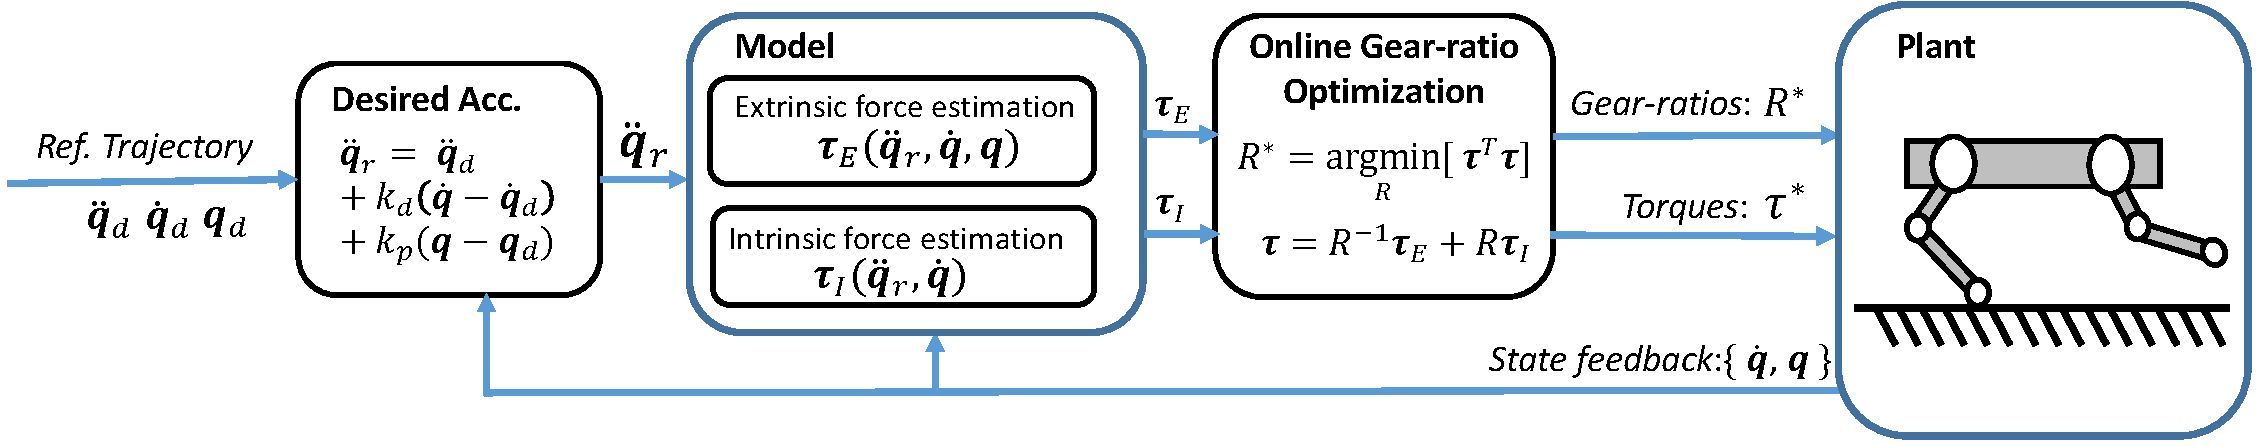
\includegraphics[width=0.99\textwidth]{Rstar_block_big.pdf}
	\caption{R* Computed Torque Controller}
	%\vspace{-10pts}
	\label{fig:Rstar_block_big}
\end{figure}

\begin{figure}[htp]
	\centering
		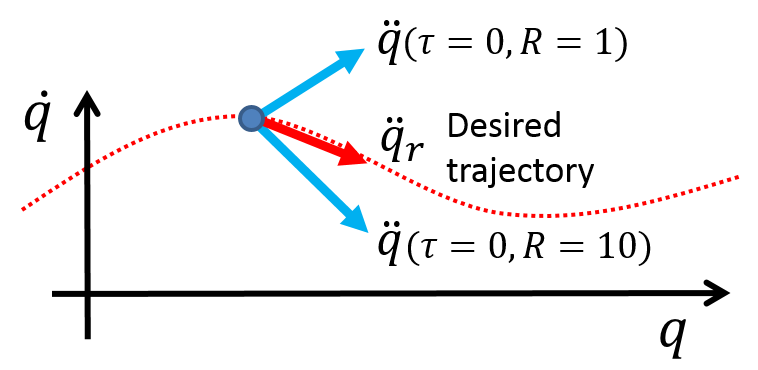
\includegraphics[width=0.40\textwidth]{dq.png}
	\caption[R* algorithm graphical interpretation]{The R* algorithm can be interpreted graphically, as selecting the gear-ratio for which the natural acceleration vector is the closet to the desired acceleration vector $\vec{\ddot{q}}_r$ (after scaling the distance with the inertia), in order to minimize the necessary torques to apply on the system.}
	\label{fig:dq}
\end{figure}

\subsection{Robust Control}
\label{sec:robustcontrol}

In general Computed Torque Control is susceptible to modeling uncertainties and disturbances. This section presents two approaches to improving robustness: Adaptation and Sliding Mode Control. 

\paragraph{Adaptation}
If the uncertainty is structured as unknown model parameters in the extrinsic dynamics, the term represented by $\vec{\tau}_E$, then traditional adaptation schemes can be used for estimating the unknown parameters. Then, if adaptation converge to the correct computed torque, then the computed best gear-ratios will also converge to the true optimal gear-ratios:
\begin{align}
	\hat{\vec{\tau}}_E \rightarrow \vec{\tau}_E 
    \quad \Rightarrow \quad 
    \hat{R}^* \rightarrow R^*
 \label{eq:adapt}
\end{align}

\paragraph{Sliding Mode Control}

Alternatively, if the uncertainty (disturbances, noise and modeling errors) is bounded, Sliding Mode Control can be applied to improving robustness. %the gear-ratio selection can also be used to minimize the torques required to guarantee convergence to the trajectory. 
Introducing intermediary variables defined as:
\begin{align}
	\vec{q}_e        = \vec{q} - \vec{q}_d  \quad \quad
	\vec{s}          = \dot{\vec{q}}_e + \lambda \vec{q}_e \quad \quad
  \vec{\ddot{q}}_r = \ddot{\vec{q}}_d - \dot{\vec{q}}_e
 \label{eq:slidingvar}
\end{align}

the computed torque, eq. \eqref{eq:eom_ndof2}, is modified to the following sliding mode control law: 
\begin{align}
	\vec{\tau} &=  R^{-1} 
	\vec{\tau}_{E}(\ddot{\vec{q}}_r,\dot{\vec{q}},\vec{q}) 
	+ R 
	\vec{\tau}_{I}(\ddot{\vec{q}}_r,\dot{\vec{q}})
    + R^{-1} G sgn( \vec{s} ) 
 \label{eq:slidingctl}
\end{align}
Convergence to the desired trajectory, despite the uncertainty, can be guaranteed using the Lyapunov function $V=\vec{s}^T \vec{s}$. The sliding condition is guarantee \cite{asada_robot_1986}, for any selected gear-ratios, if the discontinuous gain is set to:
\begin{align}
	G &= \left[ H + R^T I_a R \right] diag( \vec{k} ) \\ k_{i} &> \max \left| \left(  \left[ H + R^T I_a R \right]^{-1} \vec{d} \right)_{i} \right|
 \label{eq:slidingcond}
\end{align}
%
If the gear-ratio is selected to minimize the sliding mode torque, eq. \eqref{eq:slidingctl}, instead of the computed torque, eq. \eqref{eq:eom_ndof2}, then naturally larger gear-ratio  will be selected in response to large uncertainty. For instance, for a 1-DoF case:
\begin{align}
	R^{*} &= \operatornamewithlimits{argmin}\limits_{R} \left[ \tau^2 \right] = \sqrt{ \left | \frac{\tau_{E}(\ddot{q}_r,\dot{q},q) + | d |_{max} \, sgn( s ) }{\tau_{I}(\ddot{q}_r,\dot{q})} \right |   } 
\label{eq:rstar_sliding}
\end{align}
Hence, if no disturbance is expected ($| d |_{max}=0$) gear-ratio selection is unaffected, but when large disturbances are expected ( $| d |_{max}$ is large) torque minimization naturally leads to selecting large gear-ratios.
%


\subsection{Implementation Aspects}

\subsubsection{Numerical Online Optimization}

If some of the assumptions used in the previous section are not valid or if the gear-ratios are limited to a few discrete choices, then the optimization must be computed numerically. The minimum needed is to have a model of the inverse dynamic, which could include any non-linearity, in the form:
\begin{align}
	\vec{\tau}  = f( \vec{\ddot{q}} , \vec{\dot{q}} , \vec{q} , \vec{d} , R ) 
\end{align}
In the situation of discrete gear-ratios, this lead to a combinatorial optimization problems, adding a constraint on the gear selection in the form of:
\begin{align}
	%R^{*} &= \operatornamewithlimits{argmin}\limits_{R} \left[  \vec{\tau}^T  \vec{\tau} + \alpha \| M_{d} - M \|  \right] \quad \\
	&  R \in \{R_1,R_2, ... , R_l\} 
\end{align}
However, if the number of options $l$ is reasonably small, then every possible options can be computed quickly. For instance, for the robot presented in this paper, see Fig. \ref{fig:arm_proto}, there is 3 actuators each with 2 gear-ratio options, leading to $l=2^3=8$ possible matrix $R$.


\subsubsection{Heuristic approach to minimize gearshift}

Because the control effort during gear-shifts is neglected in the model, using the proposed controller can lead to rapid switching between gear-ratios in certain situations. To avoid this undesirable behavior, it is proposed to add hysteresis to the controller: the gear-ratio is only changed if the difference of computed torque, between using the optimal and the previously selected gear-ratio, is greater than a minimum torque threshold, and also if the elapsed time since the last change is greater than a minimum delay. 



\subsection{Rollout Optimization}




\subsection{Guarantees}


\subsubsection{Stability}

Fixed target

Convergence on desired trajectory


\subsubsection{Chattering}


If convergence is guaranteed, the zeno behavior is impossible unless the desired trajectory or point-target reside on a switching surface. 


Minimum delay on a trajectory

Proof is detailed in Appendix \ref{sec:chat1}.

Minimum delay in arbitrary situations





%%%%%%%%%%%%%%%%%%%%%%%%%%%%%%%%%%%%%%%%%%%%%%%%%%%%%%%%%%%%%%%%%%%%%%%%%%%%%%%%%%%%%%%%%%%%%%%%%%%%%%%%%%%%%%%
\newpage
\section{Trajectory planning}
\label{sec:SamplingBasedTrajectoryPlanner}



%%%%%%%%%%%%%%%%%%%%%%%%%%%%%%%%%%%%%%%%%%%%%%%%%%%%%%%%%%%%%%%%%%%%%%%%%%%%%%%%%%%%%%%%%%%%%%%%%%%%%%%%%%%%%%%%%%

\newpage

\section{Dynamic programming approach}
\label{sec:DynamicProgrammingAproach}

\begin{flushright}
\small"The true logic of this world is in the calculus of probabilities." \\ \emph{-- James Clerk Maxwell}
\end{flushright}

The proposed approach in this section is to discretize the continuous control problem into a graph search problem, with transition probability, where the discrete input actions can be considered naturally. Then dynamic programming approaches can be used to find global optimal feedback policies. 

%First, a simplified low-dimensional model of the controlled system is derived to keep the problem tractable. Second, the optimal control problem is solved using dynamic programming. Third, the resulting optimal policies are approximated with simple feedback laws, to conduct a stability analysis and also for the ease of implementation.

\subsection{Problem formulation}

The control problem of obtaining the global desired behavior is formulated as minimizing a scalar cost $J$ that is a function of the state trajectory $\vec{x}(:)$ and the inputs trajectory $\vec{u}(:)$, while constraining both states and inputs to be in their respective domains:
\begin{align}
	\operatornamewithlimits{min}\limits_{\vec{u}(:)} \; & J(\vec{x}(:),\vec{u}(:)) \\
	s.t. \quad & \vec{\dot{x}} = f(\vec{x}, \vec{u}) \quad \vec{u} \in U(\vec{x}) \quad \vec{x} \in X 
	\label{eq:min}
\end{align}

\subsection{Constraints}

The input valid set $U(\vec{x})$ is defined by allowable motor torque respecting saturation and the discrete options of gear-ratios that are feasible given actual joint velocities:
\begin{align}
	U(\vec{x}):&\\
	&\tau_i \in [ -\tau_{max,i} , \tau_{max,i} ] \;\forall\; i\\
	&k      \in \{ 0 , ... , l \} \quad\text{ such that }\quad \vec{w} = R_k \vec{\dot{q}} \in W
\end{align}
where $W$ is the set of allowable rotor velocities. The state valid set $X$ include a range of acceptable state and could exclude some regions if desired. 

\subsection{Cost function}
\label{sec:CostFunction}

Here the goal is set to minimize an additive cost function over an infinite horizon, which led to simpler time-independent control policies \cite{bertsekas_dynamic_2000}.
%
\begin{align}
	J = \lim_{ t \rightarrow \infty} \int_0^t g(\vec{x}(t),\vec{u}(t)) dt 
	\label{eq:j_lim}
\end{align}
%
Two different additive cost functions are investigated; a quadratic cost function where error is weighted against control effort:
%
\begin{align}
	g(\boldsymbol{x},\boldsymbol{u}) = \sum w^x_{ii} \; x_i^2 + \sum w^u_{ii} \; \tau_i^2
	\label{eq:g_quad}
\end{align}
%
where $w$ are weighting factors (note that there is no penalty for either gear ratio options); and a function corresponding to the minimal time problem:
%
\begin{align}
	g(\boldsymbol{x},\boldsymbol{u}) = \left \{ \begin{array}[pos]{l}	1 \quad   \text{if target not yet reached} \\ 0 \quad   \text{if target is reached} \end{array}  \right.
	\label{eq:g_time}
\end{align}
%
Note that in this section, the goal is fixed and set to zero $\boldsymbol{x}_d=\boldsymbol{0}$.


\subsection{Value Iteration}
\label{sec:VI}

A dynamic programming algorithm, also known as value iteration, is used to solve for almost exact optimal infinite horizon policies for the one-link robot. Two simplification to the problem are made, first the disturbances will be fixed to their typical values (certainty equivalence control) and second, the state space and possible control actions will be discretized.

\subsubsection{Discretization and conversion to a Stochastic Shortest Path problem}
\label{sec:ConvertionToAStocasticShortestPathProblem}

Here a evenly spaced grid of nodes is used to represent the state space. However, the equations of motion of the system can lead the system to a future state that will not be exactly a grid point corresponding to a discrete node. To solve this problem the cost-to-go of the next point is computed by interpolating the cost-to-go of the neighboring grid points based on geometric interpolation weight, see Figure \ref{fig:Probinterpolation}:
%
\begin{align}
	J(\boldsymbol{x}(t+1)) \approx \sum{ w_j J(\boldsymbol{x}_j(t+1)) } 
	\label{eq:interpol}
\end{align}
%
where the weight factors add-up to one:
%
\begin{align}
	 \sum{ w_i  } = 1
	\label{eq:w}
\end{align}
%
Thus the value iteration algorithm will have the form:
%
\begin{align}
	J_{k+1}(\boldsymbol{x}_i) =  \min_u{\left[ g(\boldsymbol{x}_i,\boldsymbol{u}) + \sum{ w_j J(\boldsymbol{x}_j(t+1))}  \right]}
	\label{eq:interpol}
\end{align}
%
\begin{figure}[htp]
	\centering
		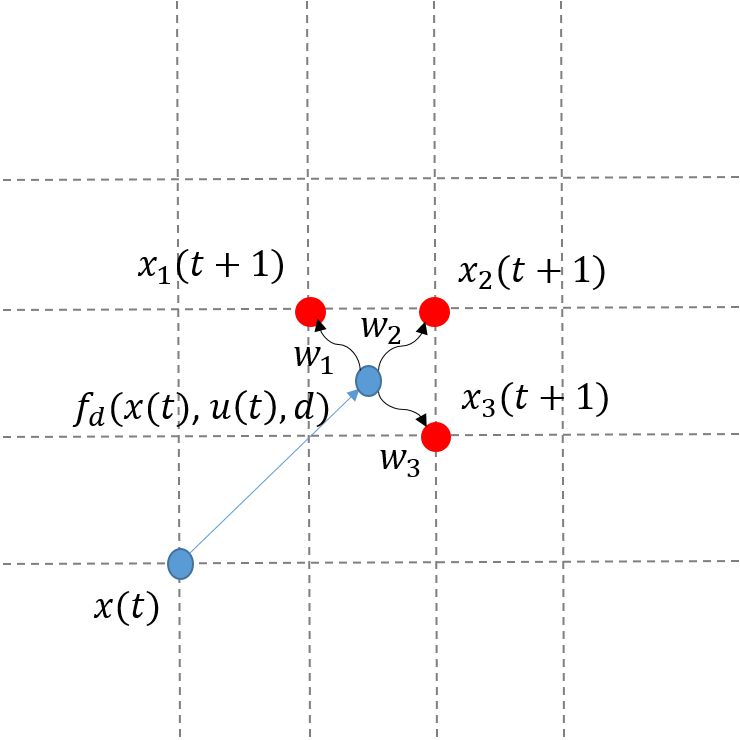
\includegraphics[width=0.40\textwidth]{interpolation.png}
	\caption{Approximation of the cost-to-go using interpolation}
	\label{fig:interpolation}
\end{figure}
%
The interpolation can also be interpreted as computing an expected value where the weight factor are probabilities. As illustrated at Figure. \ref{fig:Probinterpolation}, this scheme can also be interpreted as aggregating the continuous space state into discrete nodes with the weight factors corresponding to aggregation probabilities. Hence, the problem that is solved correspond to a stochastic shortest path problem. Note that even if the uncertainty of the system is not modeled directly, this scheme has similar effects of including a disturbance leading to an uncertainty on the state evolution of roughly the size of the grid.  
%
\begin{figure}[htp]
	\centering
		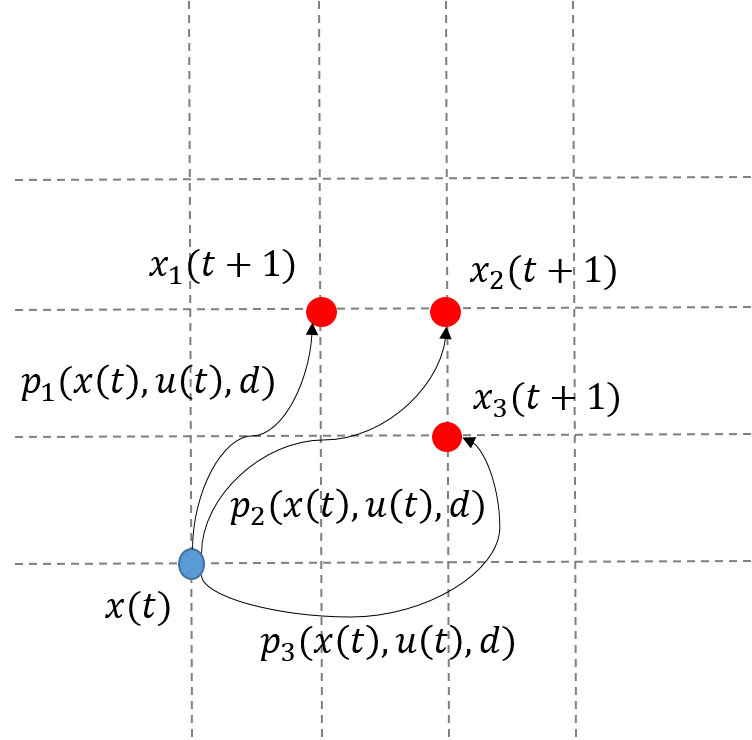
\includegraphics[width=0.40\textwidth]{Probinterpolation.png}
	\caption{Interpolation as agregation probabilities}
	\label{fig:Probinterpolation}
\end{figure}

\subsubsection{Termination conditions}
\label{sec:TerminationCondtions}

In order to guarantee the good behavior of the value iteration scheme, nodes close to the goal state are aggregated into a big cost free and absorbing termination node.  Moreover, when the equations of motion for a given state and control lead to out-of-bound states, it is considered that the system reach with a very large cost an artificial termination node with probability one. Since it is clear from the physics that there exist proper policies that can reach the termination node, and the cost is positive definite (for both the quadratic and minimum time cost functions) it is also clear that any improper policy will be associated to an infinite cost for an infinite horizon. Thus, given those conditions value iteration algorithm is guarantee to converge to the optimal cost-to-go for any initial conditions.

\subsubsection{Implementation}
\label{sec:Methodology}


The Value Iteration algorithm is implemented for two single-axis robot using a two-speed actuator. In the first case the output dynamic is a linear mass-damper system while in the second case the output is a non-linear inverted pendulum. 

The discretization parameters used are as follow: the state space is discretized into a 101 x 101 grid (101 equally spaced angles and 101 equally spaced speed values) leading to 10201 possible nodes, the actuator torque is discretized into 21 possible torque values, leading to a total of 41 possibles control actions including the gear ratio selection. The state transition is computed using a time discretization of $\Delta t$ = 0.05 sec. The interpolation weights are computed using a bivariate spline approximation. The value iterations are stopped manually when the maximum difference between $J_k$ and $J_{k+1}$ are many orders of magnitude smaller then the variations of $J$ across the state space. The computation takes on average 200-500 iterations and 2-5 minutes.

%\subsection{Reinforcement Learning}
%
%\subsubsection{Q-Learning}
%
%Next, the Q-Learning algorithm is implemented. While here in this project we have access to the model of the system, this approach would be advantageous in a real context because we could use it directly on a prototype without having a model of the robot. 
%
%The Q-learning update is:
%\begin{align}
	%Q( \boldsymbol{x} , \boldsymbol{u} ) &= Q( \boldsymbol{x} , \boldsymbol{u} ) + \alpha \left[ g(\boldsymbol{x} , \boldsymbol{u}) + \lambda J( \boldsymbol{x}_{(t+1)}  )  -  Q( \boldsymbol{x} , \boldsymbol{u} ) \right] \\
	%J( \boldsymbol{x}  ) &= \min_{\boldsymbol{u}} Q( \boldsymbol{x}, \boldsymbol{u} )
   %\end{align}
   %
%This update is conducted for each set of $\left[ \boldsymbol{x}_{(t)}  , \boldsymbol{u}_{(t)}  , \boldsymbol{x}_{(t+1)}   \right]$ collected using simulated experiments. The controller used for the experiment is $\epsilon$-greedy, i.e. $\epsilon$ fraction of the time it picks a random action, else it is using the optimal action so far ( $ u(\boldsymbol{x})  = arg\min_{\boldsymbol{u}} Q( \boldsymbol{x}, \boldsymbol{u} ) $ ). The training is done as follow: first conduct a 10 sec simulation with the $\epsilon$-greedy controller, then go through the collected state-action pairs and conduct a Q-values update for each data-point, then start again.

%\paragraph{Numerical results}
%\label{sec:NumericalResults}
%
%This approach was found to be practical only for very simple robots. For instance, one degree of freedom lead to two states (position and speed). If each of those variable is discretized into 100 levels, the total number of possible states is 10000. Then if we use 10 possible levels of torque times two gear ratios we have 20 possibles action. Hence, we must keep track of 200000 Q-values, and we need to visit each of those values multiple time to converge. For more complex systems the brute force look-up table approach is thus even less tractable then value iteration.
%
%\begin{figure}[hpt]
        %\centering
				%\subfloat[Cost-to-go]{
				%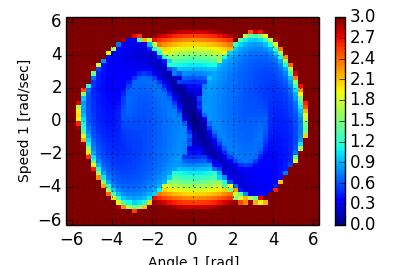
\includegraphics[width=0.32\textwidth]{Q_1_J2.png}}
        %\subfloat[Policy for torque]{
				%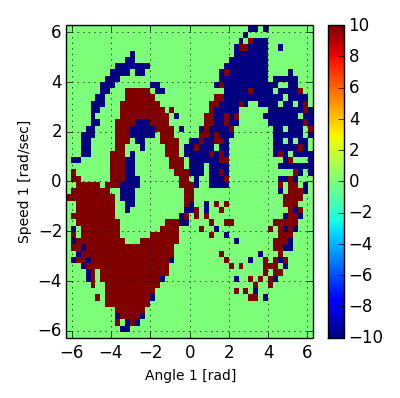
\includegraphics[width=0.25\textwidth]{Q_1_u0.png}}
				%\subfloat[Trajectory using the learned policy]{
				%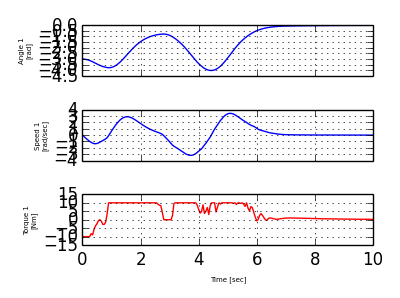
\includegraphics[width=0.32\textwidth]{Q_1_xu.png}}
       %\caption{Results with Q-Learning for a 1-DOF robot after thousands of simulated experiments}
			%\label{fig:Q}
%\end{figure}
%
%The results are illustrated at Fig. \ref{fig:Q}. For this experiment, the set of possible action was limited to only 3 torque levels, to reduce the necessary computation time. After thousands of simulated experiment, it was possible to see a cost-to-go mapping similar to the one obtained with value iteration. Interesting point is that for some region of the state-space, the cost-to-go is different (still equal to the initialization value) because those zones were never visited during the experiments. Also, even if the state-space exploration was far from complete, the controller obtained at this point was still able to bring the robot on the target.
%
%
%\subsubsection{Feature based reinforcement learning}
%
%
%In this section, instead of learning a look-up table for the cost-to-go or Q-values, an approximation of the cost-to-go using features and a small set of weights is learned. This approach as the advantage of scaling more easily to complex robots and to avoid Bellman`s "curse of dimensionality". The approximation will be done directly on the cost-to-go function:
%
%\begin{align}
	%\hat{J}(\boldsymbol{x}) &= \sum_i  w_i  f_i(\boldsymbol{x})  
	%\label{eq:Qhat}
%\end{align}
%
%With the weight update:
%\begin{align}
	%w_i =w_i + \alpha \left[ g(\boldsymbol{x} , \boldsymbol{u}) + \lambda \hat{J}(\boldsymbol{x}_{(t+1)})  -  \hat{J}(\boldsymbol{x}) \right] f_i(\boldsymbol{x},\boldsymbol{u}) 
%\end{align}
%
%This correspond to temporal-difference learning scheme. During the learning phase, the controller $\epsilon$-greedy is again used. One difference is that since only the cost-to-go is estimated, the greedy policy needs to do a one-step look-ahead to select the best action, i.e. $ u(\boldsymbol{x})  = arg\min_{\boldsymbol{u}} \left[ g(\boldsymbol{x} , \boldsymbol{u}) + \lambda \hat{J}(\boldsymbol{x}_{(t+1)}) \right] $. Note that with this approach, since we are doing both policy evaluation and policy improvement simultaneously, we will converge to a local minimum, unlike Q-learning where we are guarantee to find the global optimum if we run it for long enough.
%
%
%\paragraph{Feature design}
%\label{sec:features}
%
%The features were picked using physical intuition from the dynamical system. Since the cost-to-go function needs to represent how far away the system is from the goal, in term of future cost with the optimal behavior, one good indicator in the energy level. If the actual energy level is very different from the goal energy level, then a lot of control effort will be required to change that and there is no way around it. So the first feature is :
%%
%\begin{align}
	%f_1(\boldsymbol{x}) &=  | energy( \boldsymbol{x} )  - energy( \boldsymbol{x}_{target} ) |
%\end{align}
%%
%However, simply having the correct energy level is not enough to reach the goal. We also need to penalize position error and velocity leading away from the goal, both which will make the system incur additional cost. In order to do that, sliding variable are used, one for each joint of the robot. A sliding variable is the combination of a position error and a velocity error into a single scalar:
%%
%\begin{align}
	%s_i &=  \dot{q_e}  + \lambda q_e
%\end{align}
%%
%where $q_e$ is a joint position error and $\dot{q_e}$ is a joint velocity error. If $s_i$ is very small then the error on this joint is converging toward zero, hence this can be used to know if the system is in a good/bad situation. So for the 1-DOF robot, only two features are used: the absolute error on energy level and the absolute value of the sliding variable. Three variables thus parametrize $\hat{J}$ (the third one correspond to an offset). For the 2-DOF robot, only an additional sliding variable is added as a feature to account for the additional joint.
%
%
%\paragraph{Numerical results}
%\label{sec:NumericalResults}
%
%Fig. \ref{fig:aaa} shows the first experiment, with the initial weights set so the initial cost-to-go is only the energy error. We can see that this is not enough and the controller fail to stabilize the robot. However, after only 20 experiments, the weights had converged and the resulting controller was doing a good job of bringing the robot to the target. Note that the approximated cost-to-go is not too far from the cost-to-go obtained using value iteration, at least considering only 3 parameters are used. 
%
%\begin{figure}[hp]
        %\centering
				%\subfloat[Approximated Cost-to-go]{
				%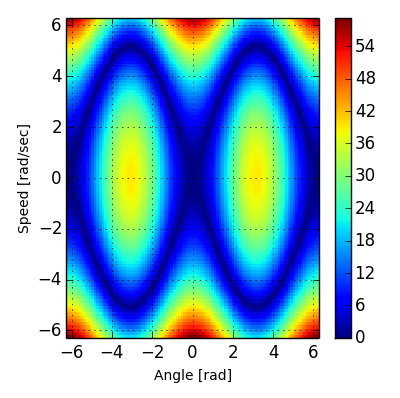
\includegraphics[width=0.28\textwidth]{eG1_J0.png}}
        %\subfloat[Phase plane trajectory]{
				%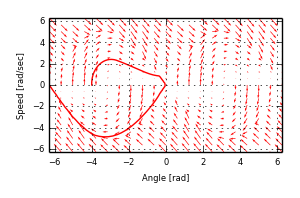
\includegraphics[width=0.32\textwidth]{eG1_pp0.png}}
				%\subfloat[State and input trajectory]{
				%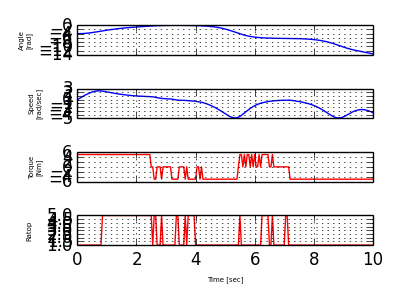
\includegraphics[width=0.32\textwidth]{eG1_xu0.png}}
       %\caption{Results of 2-features learning after 1 experiment (controller failed to stabilize the goal) }
			 %\label{fig:aaa}
%\end{figure}
%
%\begin{figure}[hp]
        %\centering
				%\subfloat[Approximated Cost-to-go]{
				%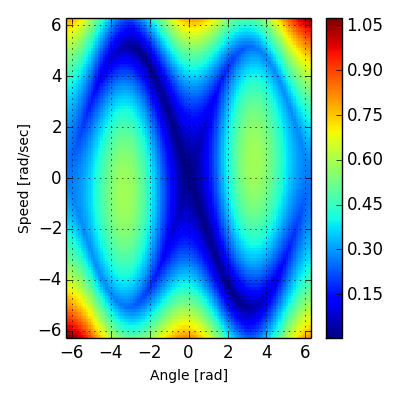
\includegraphics[width=0.28\textwidth]{eG1_J20.png}}
        %\subfloat[Phase plane trajectory]{
				%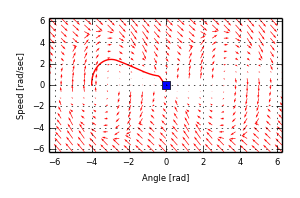
\includegraphics[width=0.32\textwidth]{eG1_pp20.png}}
				%\subfloat[State and input trajectory]{
				%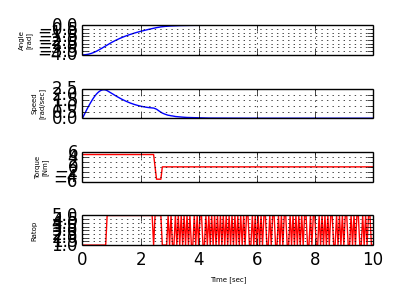
\includegraphics[width=0.32\textwidth]{eG1_xu20.png}}
       %\caption{Results of 2-features learning after 20 experiments (weight converged)}
			%\label{fig:aaa}
%\end{figure}
%
%Similar results were obtained for the 2-DOF robot, see the youtube video at \url{https://youtu.be/JJejTTy1-bU}. 
%
%Note: I tried adding a lot more features, for instance directly the states, the square of the states, sin/cos of the states, etc. However, no meaningful improvement was obtained by doing so.
%
%

\subsection{Numerical results}

\subsubsection{Linear 1-DoF robot}
Fig. \ref{fig:J} to \ref{fig:u1} illustrate the numerical results of the Value Iteration algorithm for the linear mass-damper output case. Three different cost functions are explored, a quadratic cost function, a mininimum time cost and minimum energy case which is simply a special case of the quadratic cost where weight are sets to drastically penalize control inputs over state error. The absence of color indicates states with no solution (a constraint will be violated for any possible control actions). Fig. \ref{fig:phase_plane} shows the closed loop behavior of the system in the phase plane when the optimal policy is applied.
%
\begin{figure}[H]
        \centering
				\subfloat[Minimum time]{
        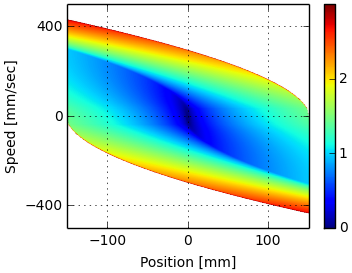
\includegraphics[width=0.32\textwidth]{Jt.png}
				\label{fig:J_time}}
        \subfloat[Quadratic cost]{
				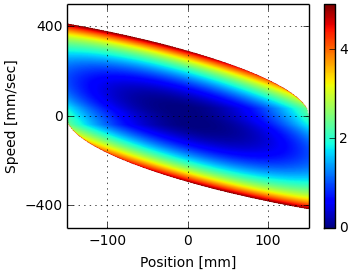
\includegraphics[width=0.32\textwidth]{Jq.png}%J_LQR.png
				\label{fig:J_LQR}}
				\subfloat[Minimum energy]{
				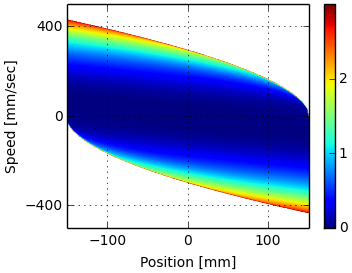
\includegraphics[width=0.32\textwidth]{Je.png}
				\label{fig:J_energy}}
        \caption{Optimal cost-to-go $J^*$}\label{fig:J}
\end{figure}
%
\begin{figure}[H]
        \centering
				\subfloat[Minimum time]{
        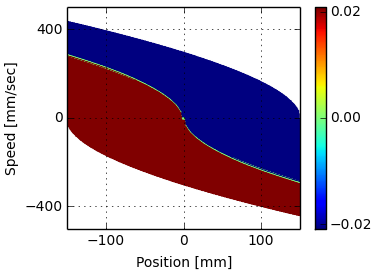
\includegraphics[width=0.32\textwidth]{u1t.png}
				\label{fig:u0_time}}
        \subfloat[Quadratic cost]{
				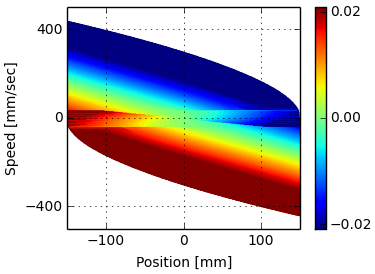
\includegraphics[width=0.32\textwidth]{u1q.png}
				\label{fig:u0_LQR}}
				\subfloat[Minimum energy]{
				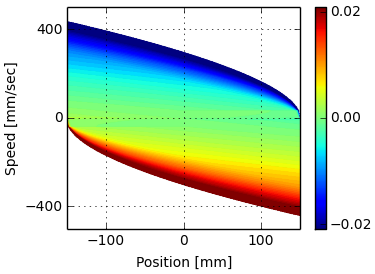
\includegraphics[width=0.32\textwidth]{u1e.png}
				\label{fig:u0_energy}}
        \caption{Optimal policy for the continuous torque command $u_1$ [Nm]}\label{fig:u0}
\end{figure}
%
\begin{figure}[H]
        \centering
				\subfloat[Minimum time]{
        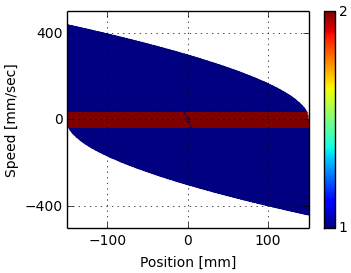
\includegraphics[width=0.32\textwidth]{u2t.png}
				\label{fig:u1_time}}
        \subfloat[Quadratic cost]{
				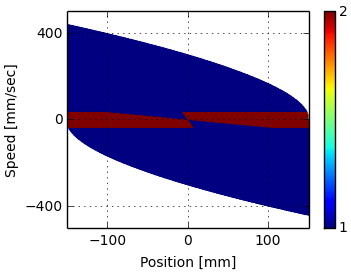
\includegraphics[width=0.32\textwidth]{u2q.png}
				\label{fig:u1_LQR}}
				\subfloat[Minimum energy]{
				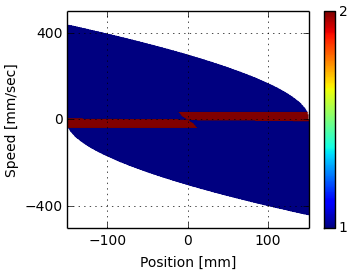
\includegraphics[width=0.32\textwidth]{u2e.png}
				\label{fig:u1_energy}}
        \caption{Optimal policy for the mode selection $u_2$}\label{fig:u1}
\end{figure}
%
\begin{figure}[H]
        \centering
				\subfloat[Minimum time]{
        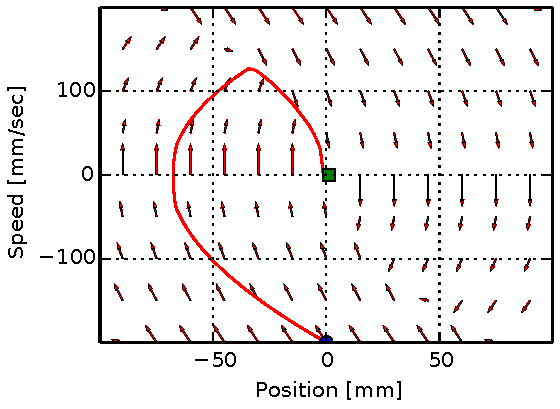
\includegraphics[width=0.32\textwidth]{ppt.pdf}
				\label{fig:phase_plane_time}}
        \subfloat[Quadratic cost]{
				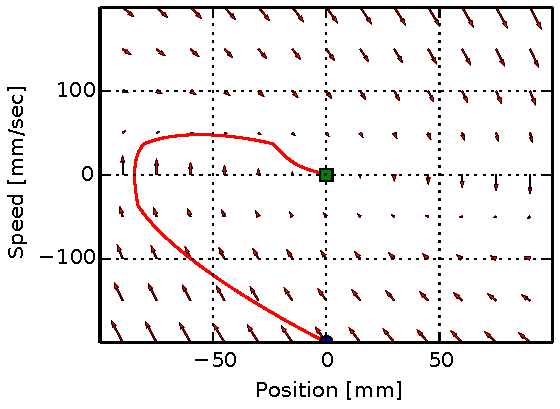
\includegraphics[width=0.32\textwidth]{ppq.pdf}
				\label{fig:phase_plane_LQR}}
				\subfloat[Minimum energy]{
				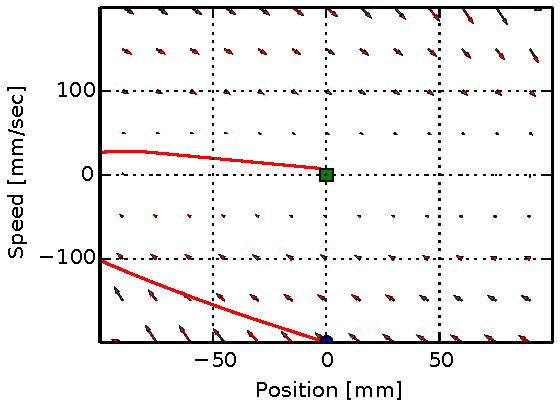
\includegraphics[width=0.32\textwidth]{ppe.pdf}
				\label{fig:phase_plane_energy}}
        \caption[Closed loop behavior in the phase plane]{Closed loop behavior with the optimal policy illustrated in the phase plane}\label{fig:phase_plane}
\end{figure}

\paragraph{Minimum time}
\label{sec:MinimumTime}
For the minimum time problem, the optimal policy is a bang-bang law for the torque and always using highly-geared mode when possible. Note that the bang-bang switching curve accounts for the fact the large gear ratio will be used during the final part of the trajectory.

\paragraph{Quadratic cost}
\label{sec:QuadraticCost}
For the quadratic cost, the gear-ratio selection optimal policy is almost as simple as the minimum time problem except for small features in quadrant II and IV. The more interesting result comes from the continuous torque control law, the gains when using the large reduction ratio are larger than those when using the small reduction ratio. This results in the controller taking action mainly at low speed when its actions have the biggest impacts on the system, and lead to a highly non-linear closed-loop behavior.

\paragraph{Minimum energy}
\label{sec:MinimumEnergy}
For the minimum energy controller, interestingly the mode selection policy is not trivial even for this simple linear model.  This shows that it does not take much complexity to have non-trivial optimal policies for hybrid systems. Here, the large reduction ratio is used almost only for braking, and in quadrant II and IV the small reduction ratio is used even at low speed to coast with low viscous resistance. Also globally the gains are much lower than the other controllers except for zones where it is necessary to use energy to stay in the domain. 

\subsubsection{Non-linear 1-DoF robot}

Figure \ref{fig:J} illustrates the computed optimal cost-to-go for the inverted pendulum system for both a minimal time goal and a quadratic cost minimization. Figure \ref{fig:u0} shows the optimal torque policy and Figure \ref{fig:u1} shows the optimal gear selection policy. The resulting closed loop behavior is illustrated in the phase plane at Figure \ref{fig:phase_plane}. Figure \ref{fig:phase_plane} also shows closed-loop state trajectories and control inputs for a simulation starting at $q$ = -2 rad.

\begin{figure*}[htpb]
        \centering
				\subfloat[Minimum time]{
        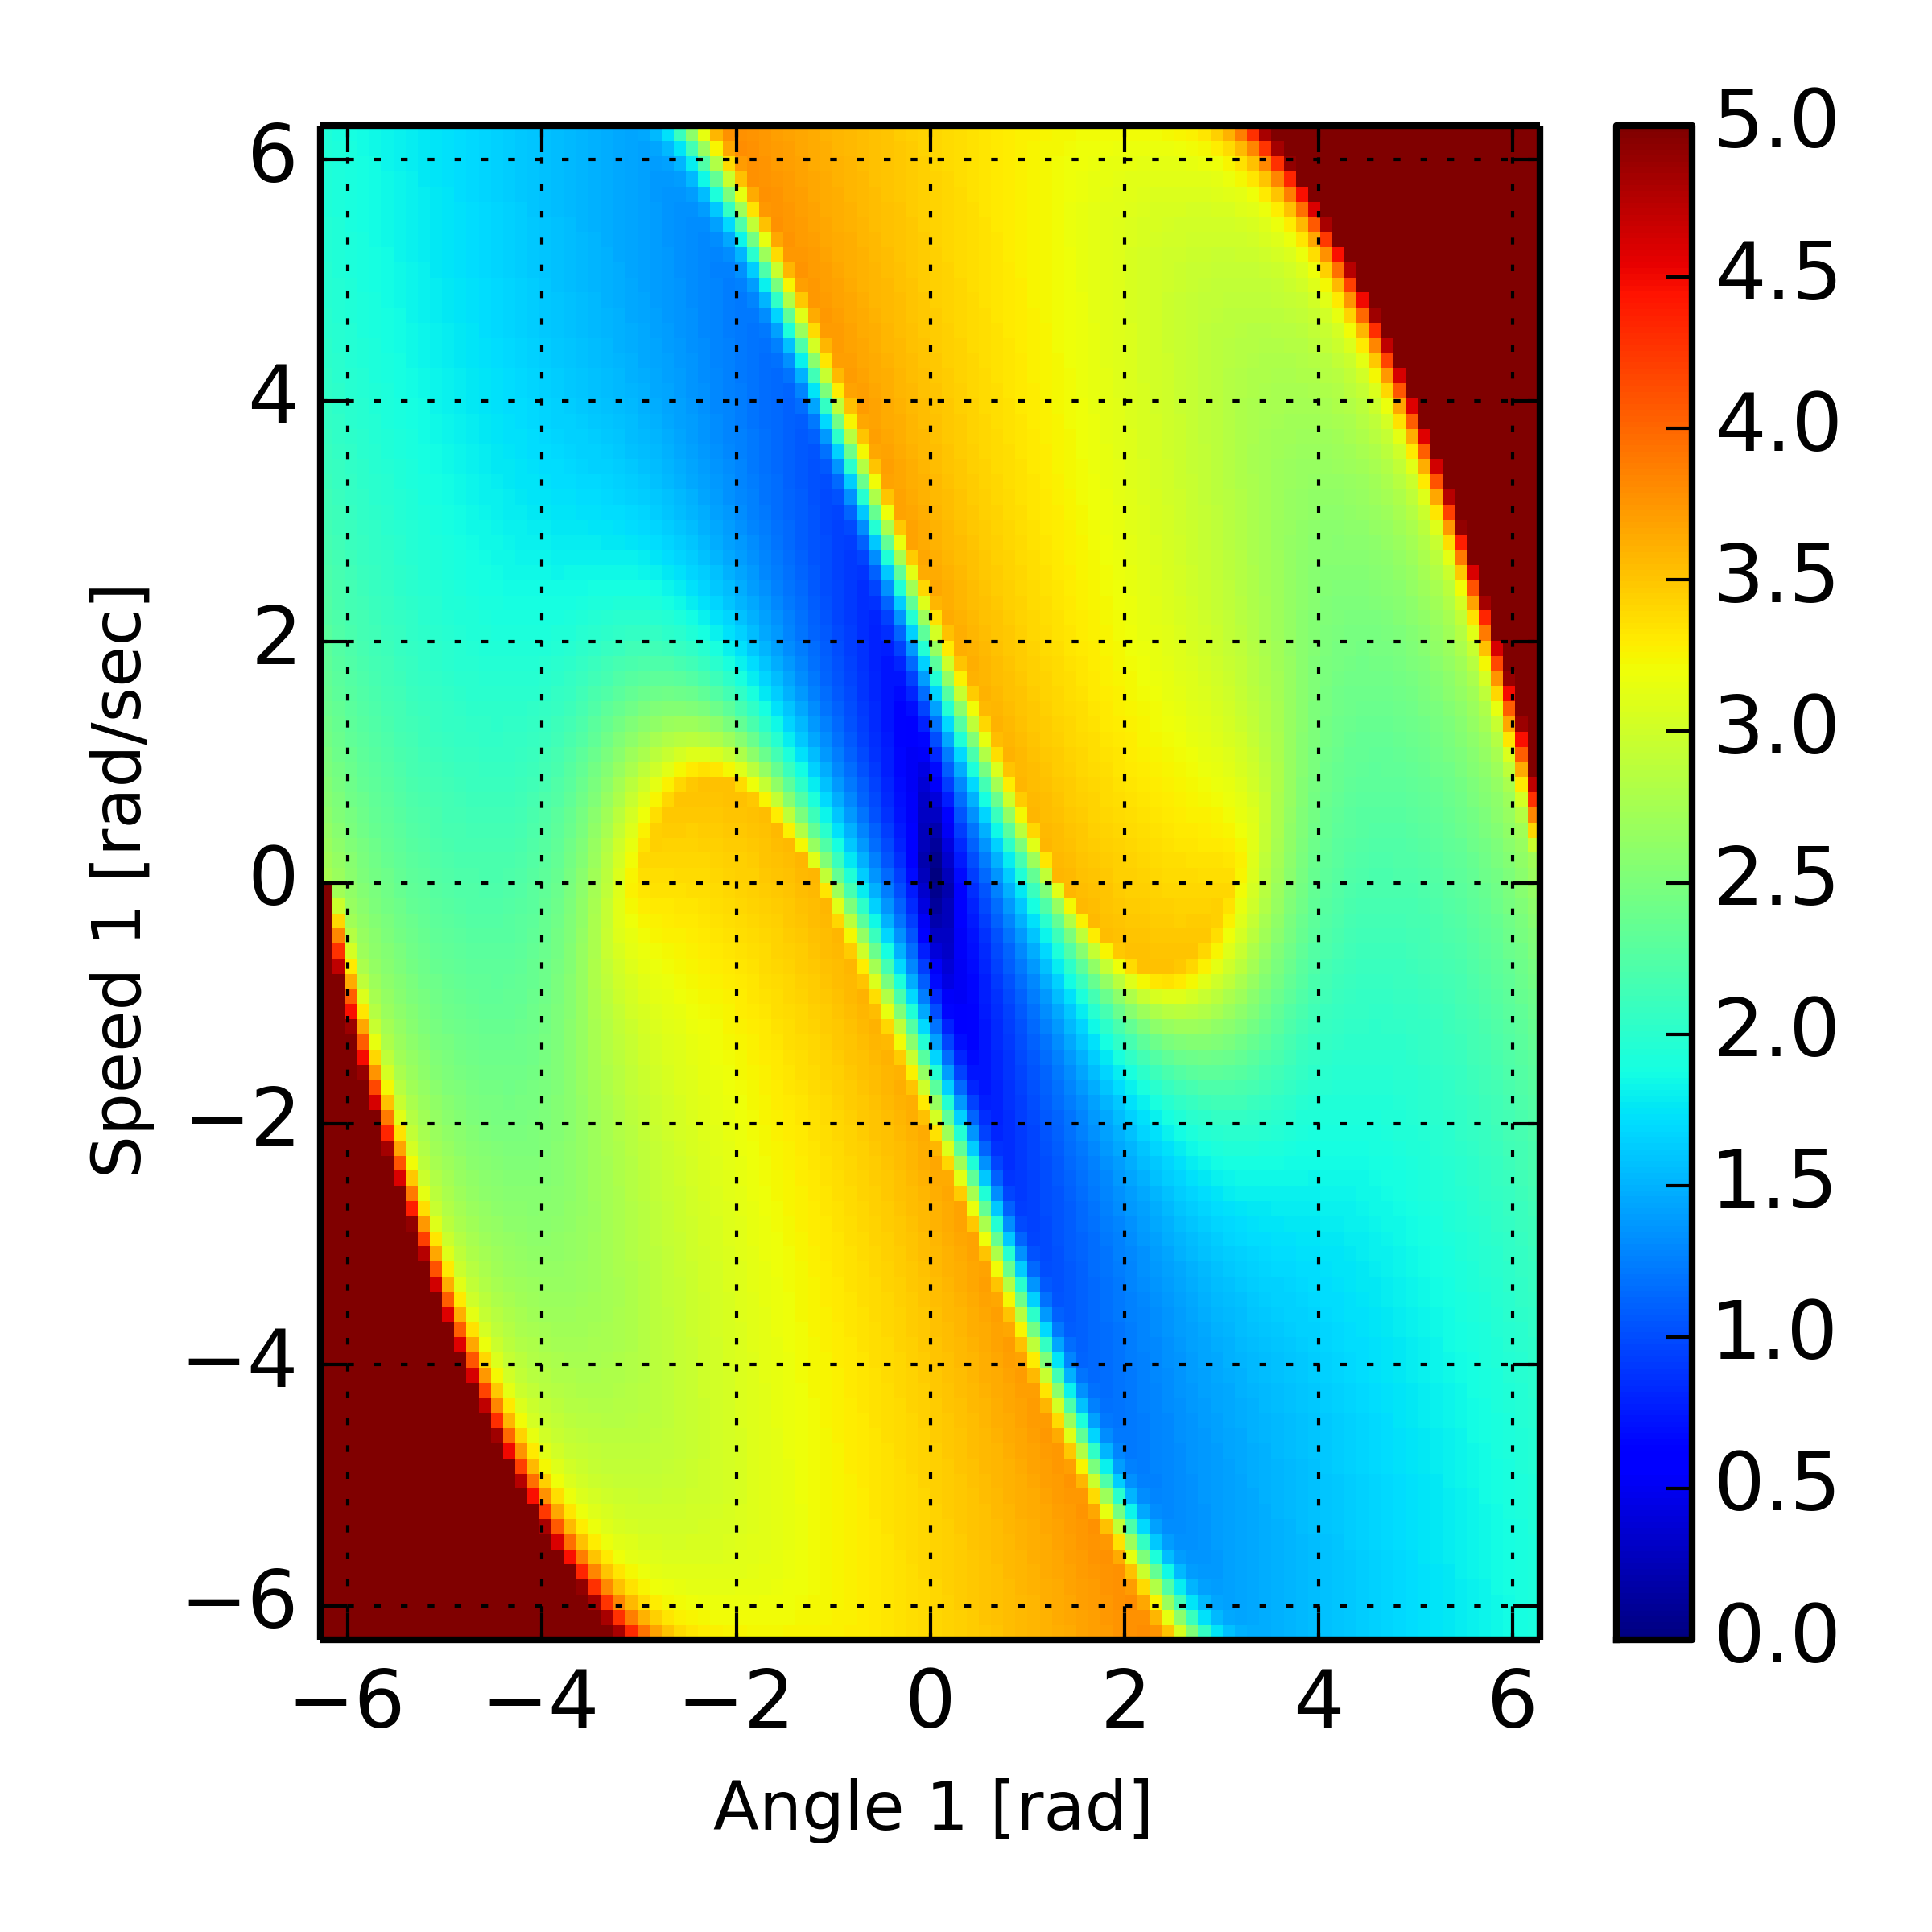
\includegraphics[width=0.48\textwidth]{J_time.png}
				\label{fig:J_time}}
        \subfloat[Quadratic cost]{
				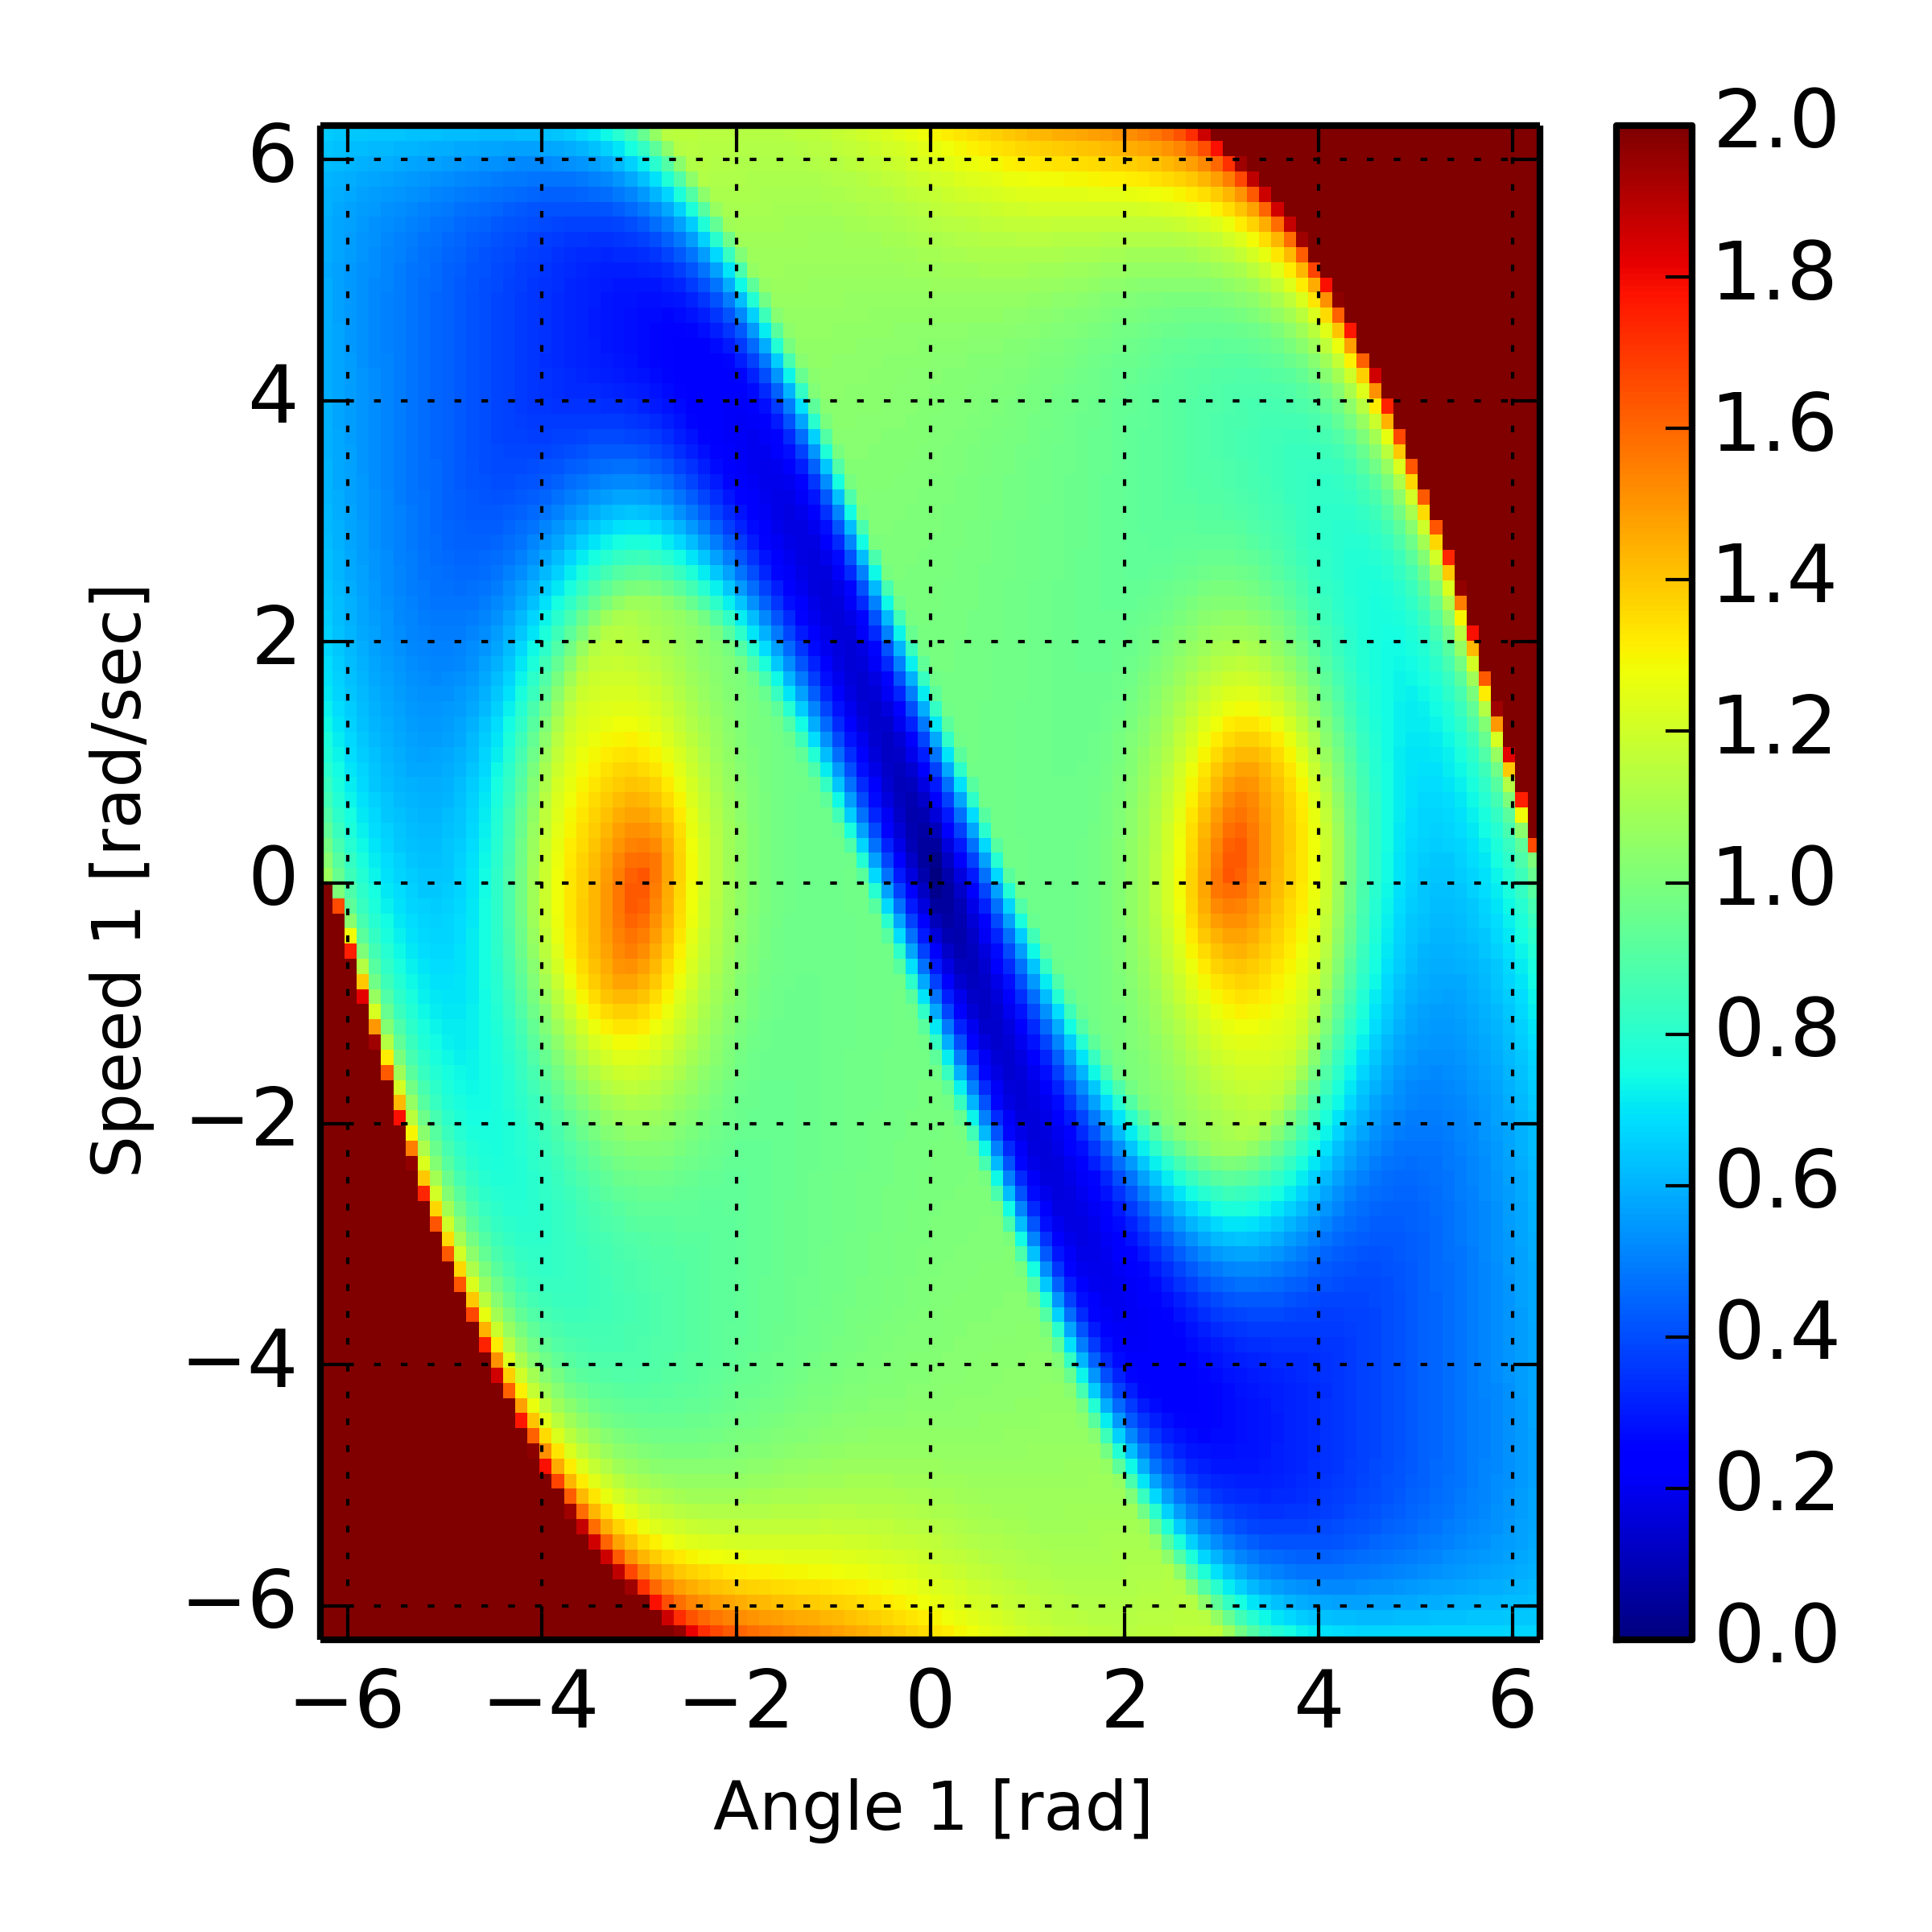
\includegraphics[width=0.48\textwidth]{J_quadratic.png}%J_LQR.png
				\label{fig:J_LQR}}
        \caption{Optimal cost-to-go $J^*$}\label{fig:J}
\end{figure*}

\begin{figure*}[htpb]
        \centering
				\subfloat[Minimum time]{
        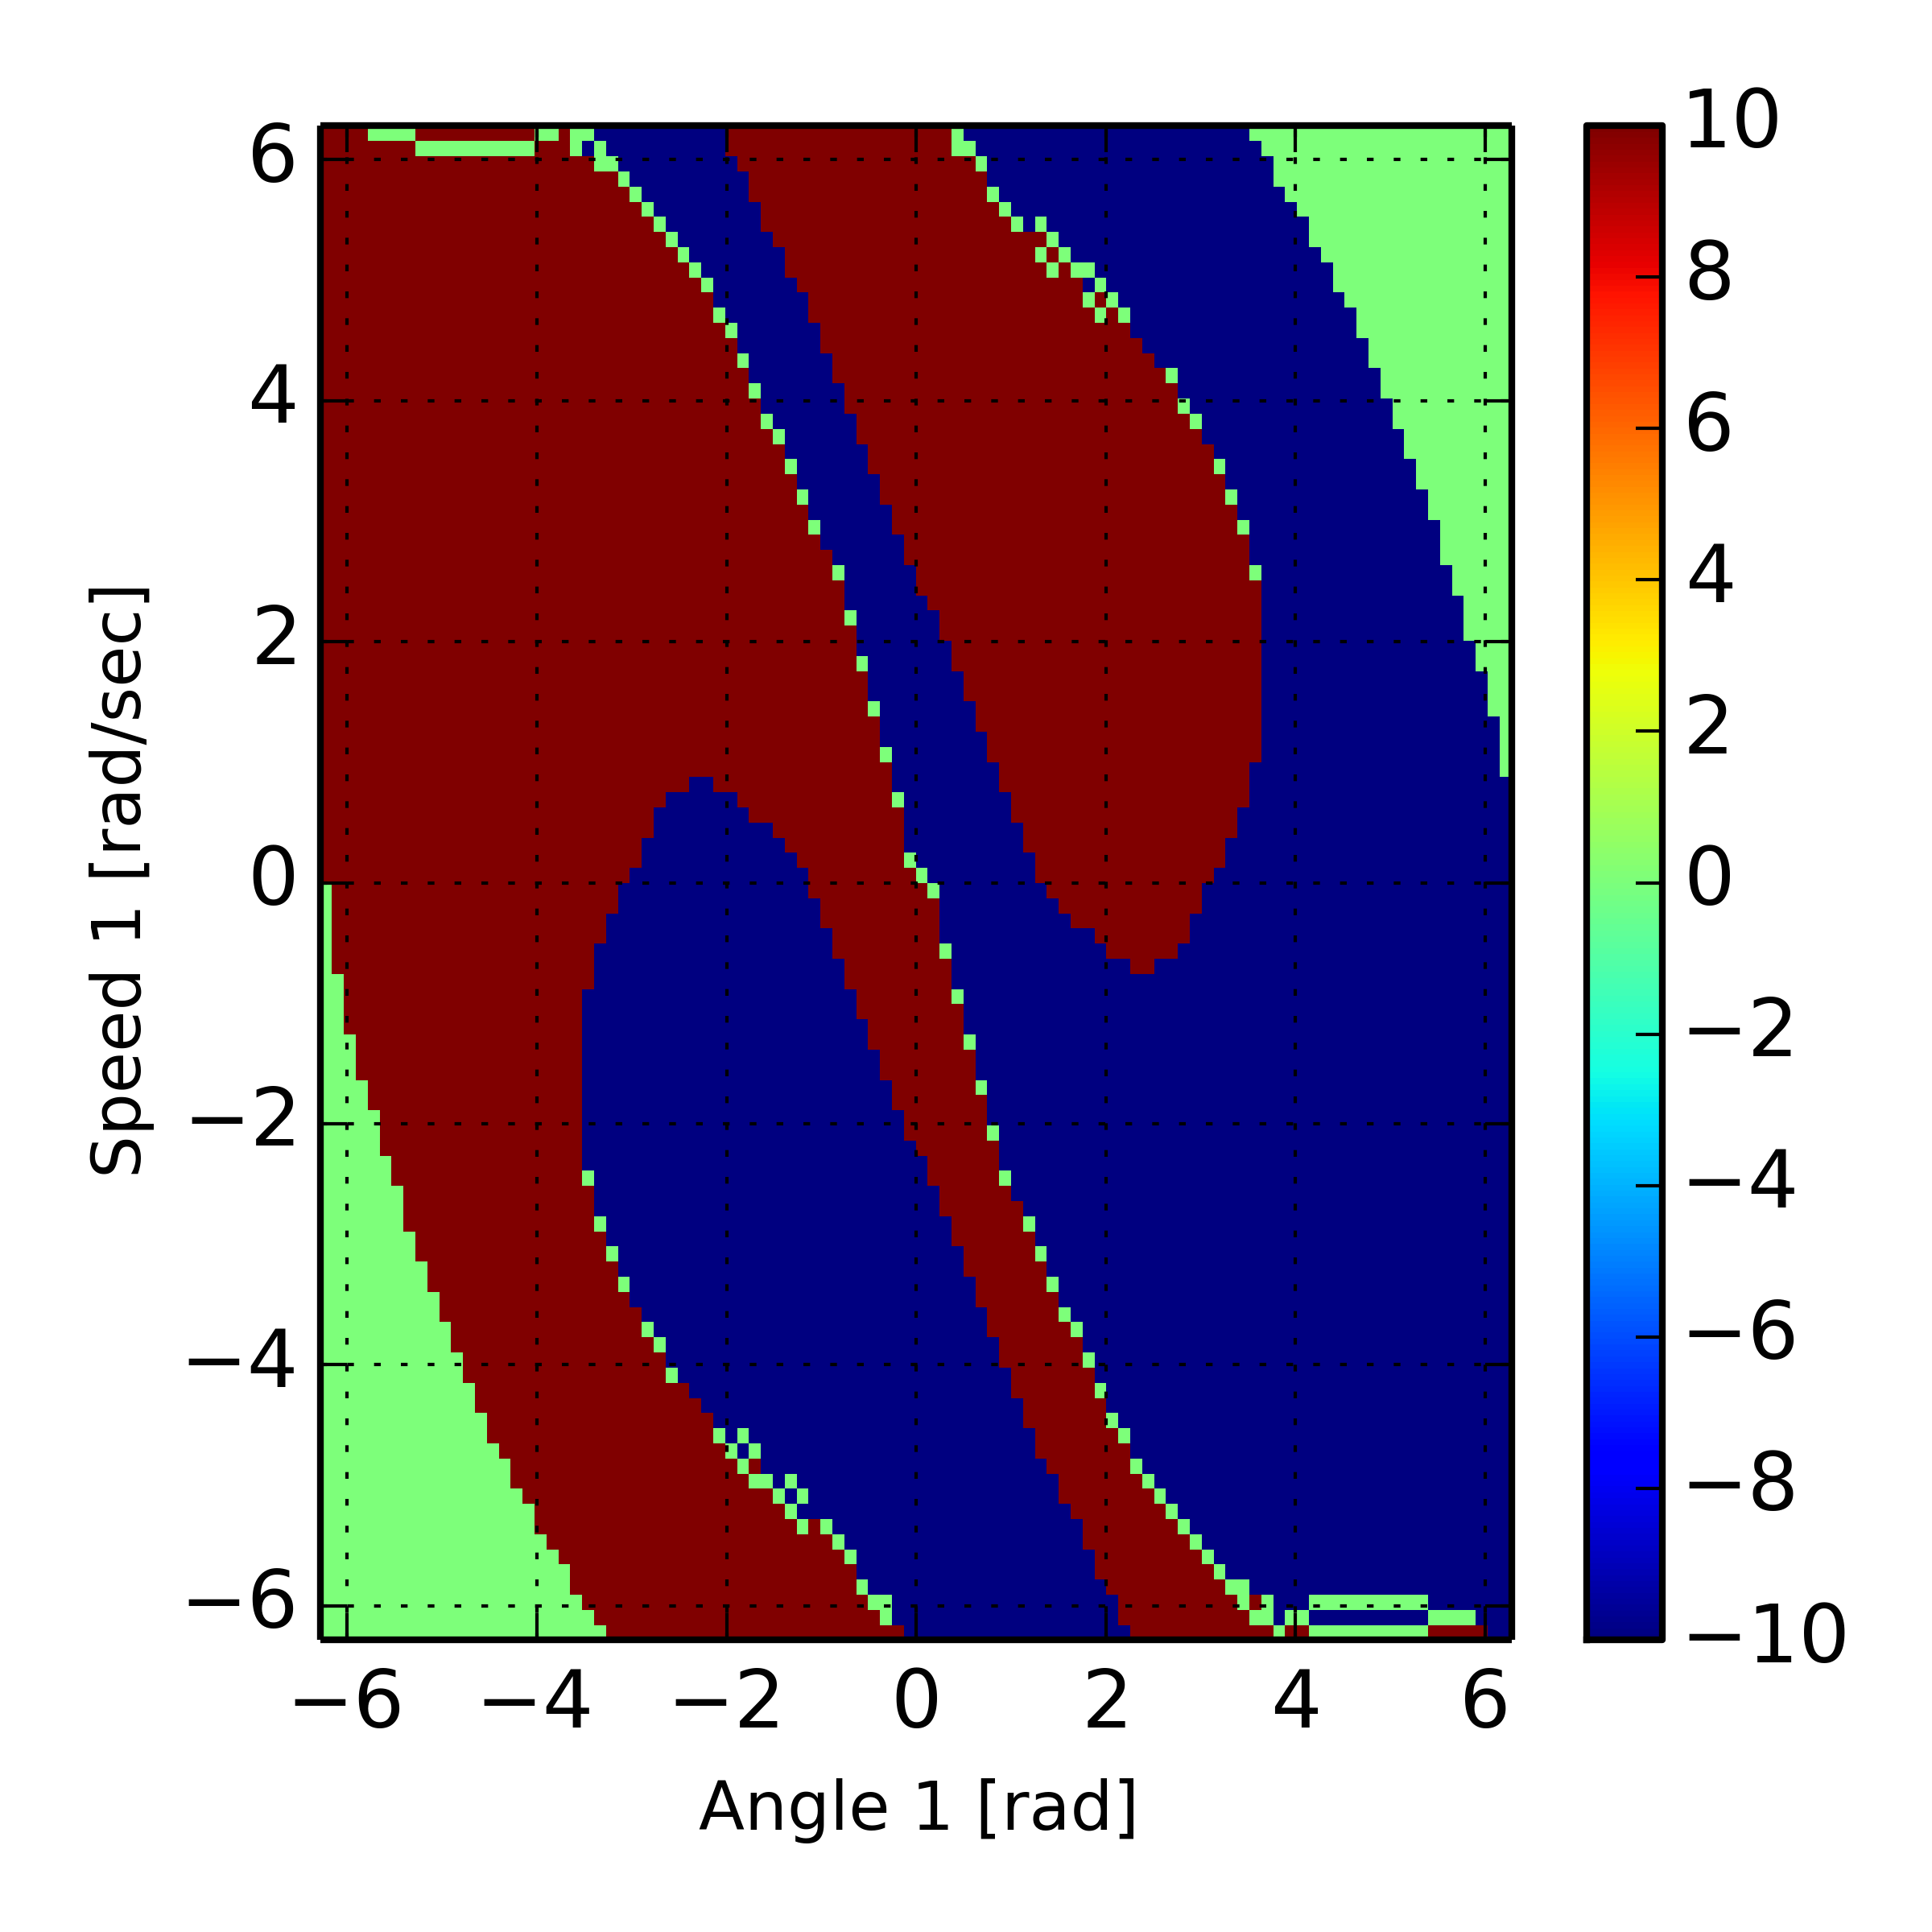
\includegraphics[width=0.48\textwidth]{u0_time.png}
				\label{fig:u0_time}}
        \subfloat[Quadratic cost]{
				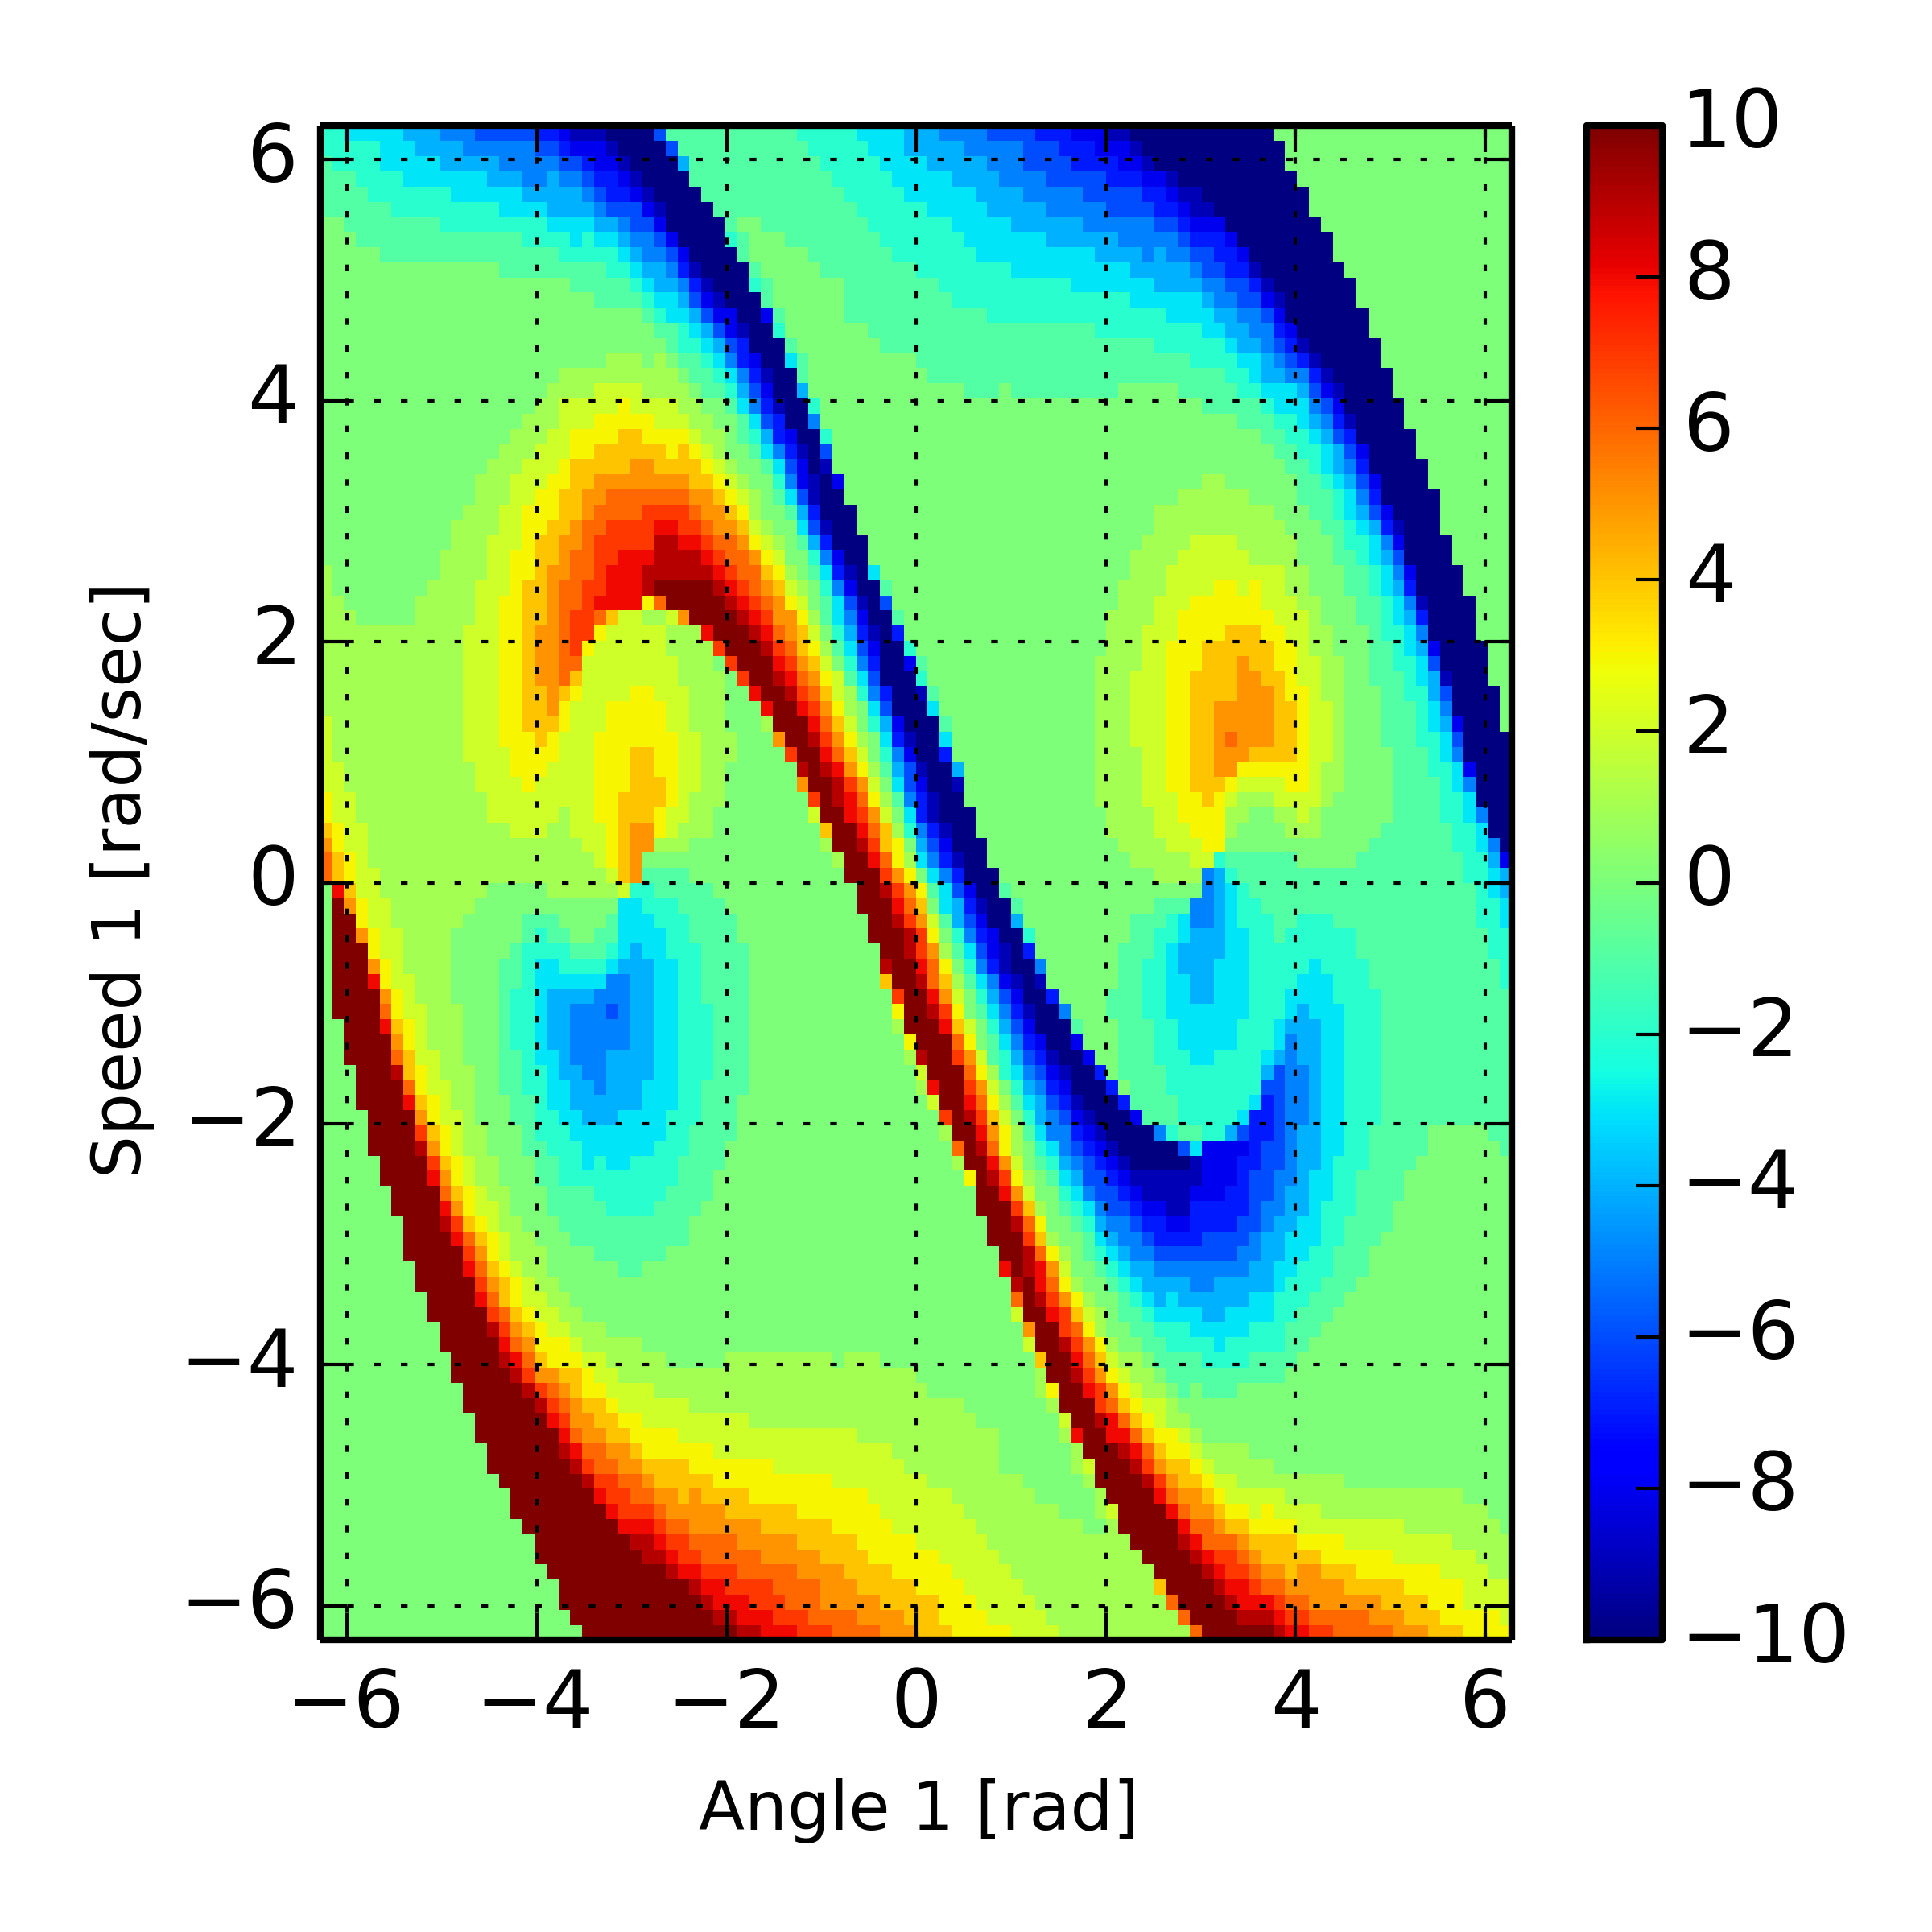
\includegraphics[width=0.48\textwidth]{u0_quadratic.png}
				\label{fig:u0_LQR}}
        \caption{Optimal policy for the continuous torque command $\tau$ [Nm]}\label{fig:u0}
\end{figure*}

\begin{figure*}[htpb]
        \centering
				\subfloat[Minimum time]{
        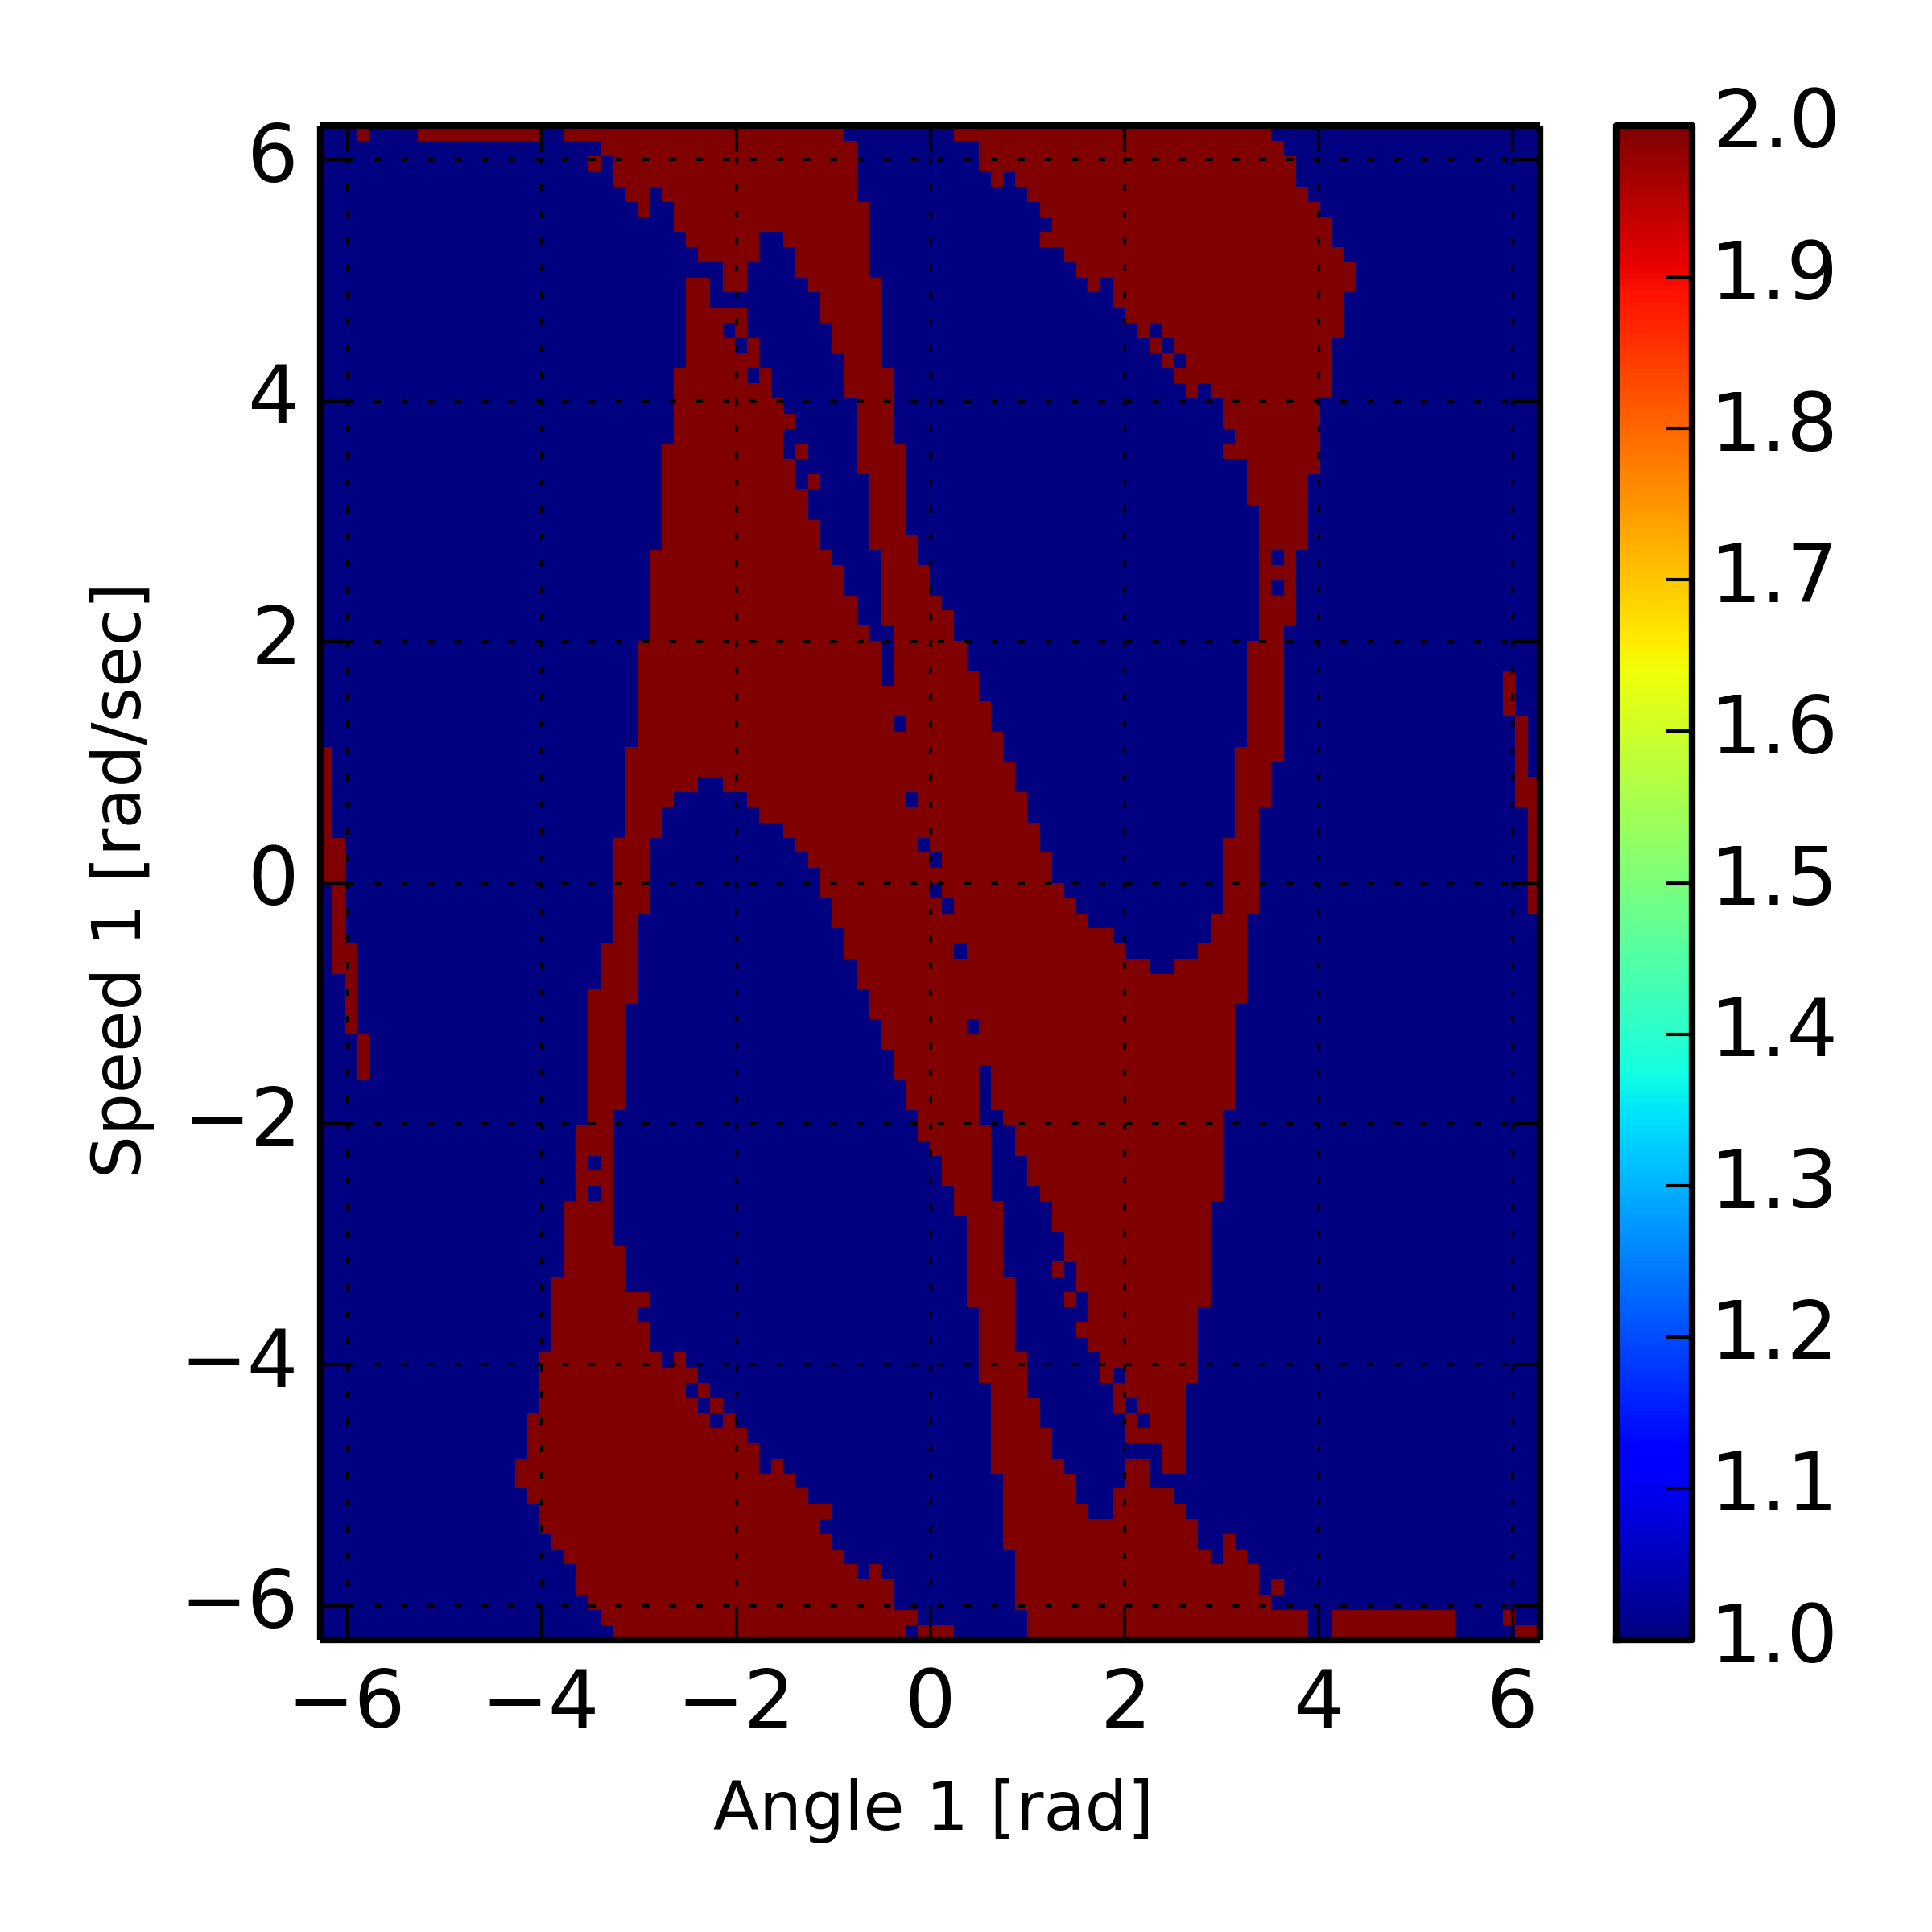
\includegraphics[width=0.48\textwidth]{u1_time.png}
				\label{fig:u1_time}}
        \subfloat[Quadratic cost]{
				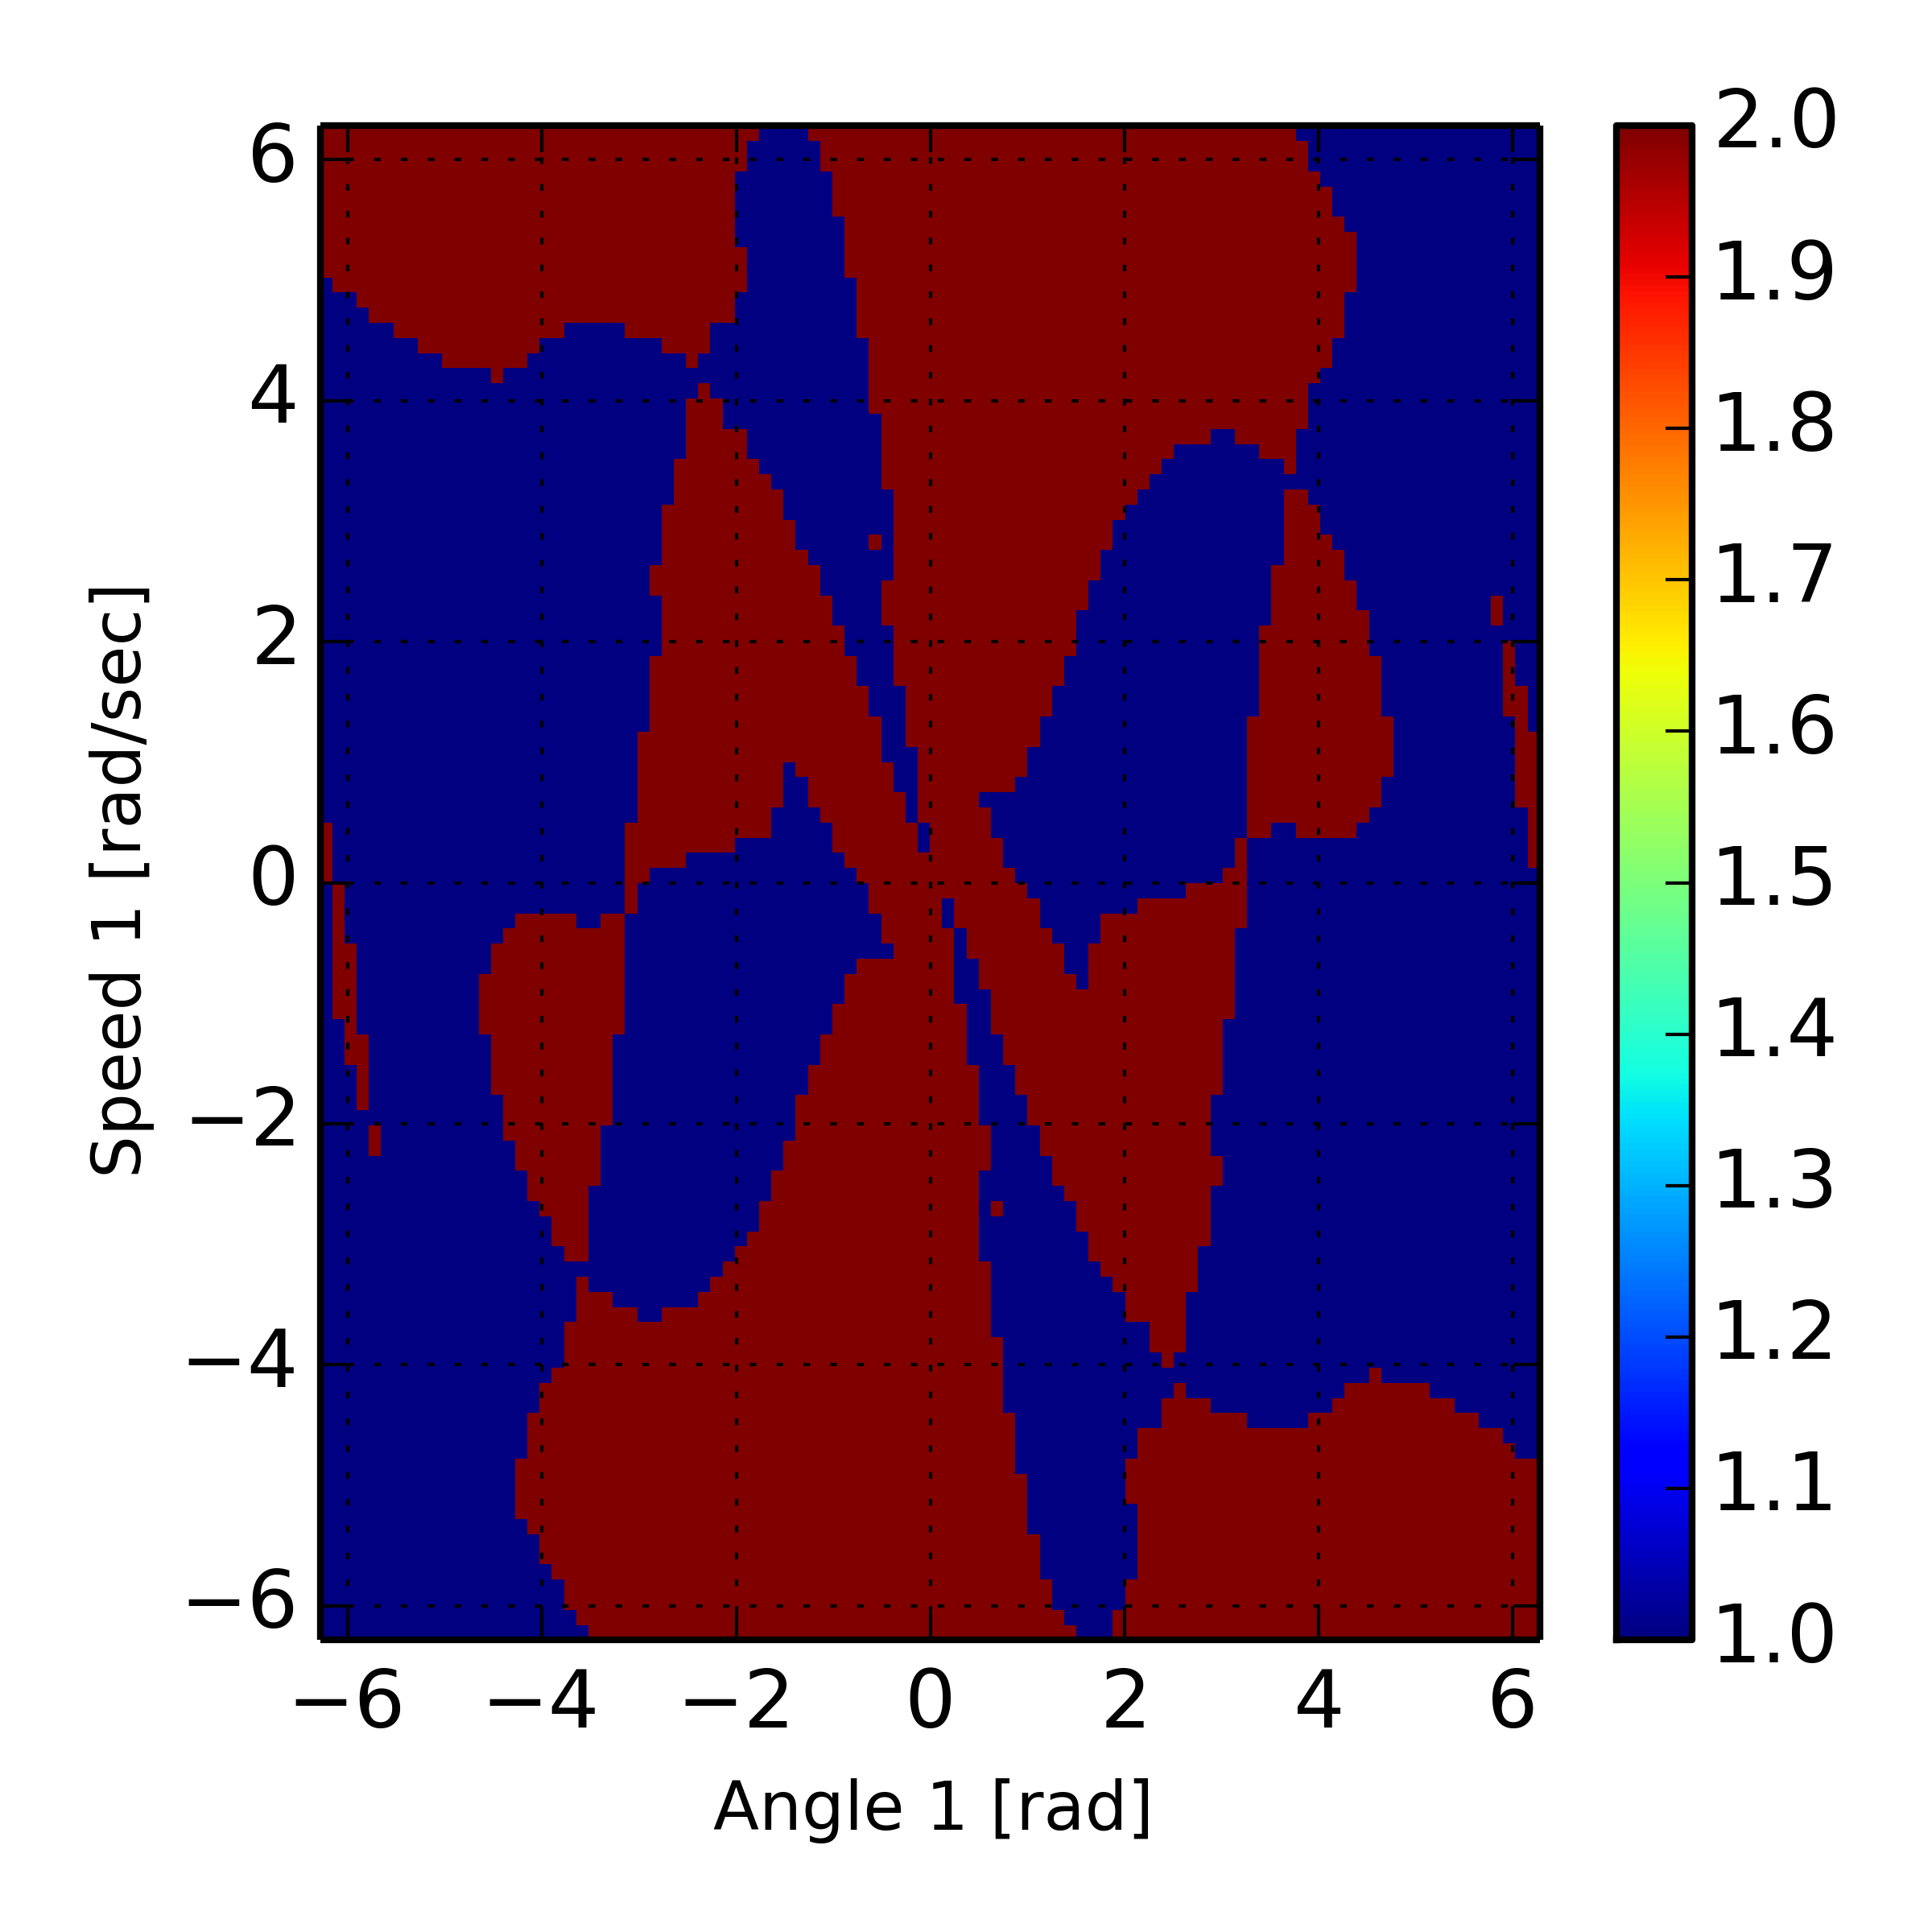
\includegraphics[width=0.48\textwidth]{u1_quadratic.png}
				\label{fig:u1_LQR}}
        \caption{Optimal policy for the discrete gear selection $k \in [1,2]$}\label{fig:u1}
\end{figure*}

\begin{figure*}[htpb]
        \centering
				\subfloat[Minimum time]{
        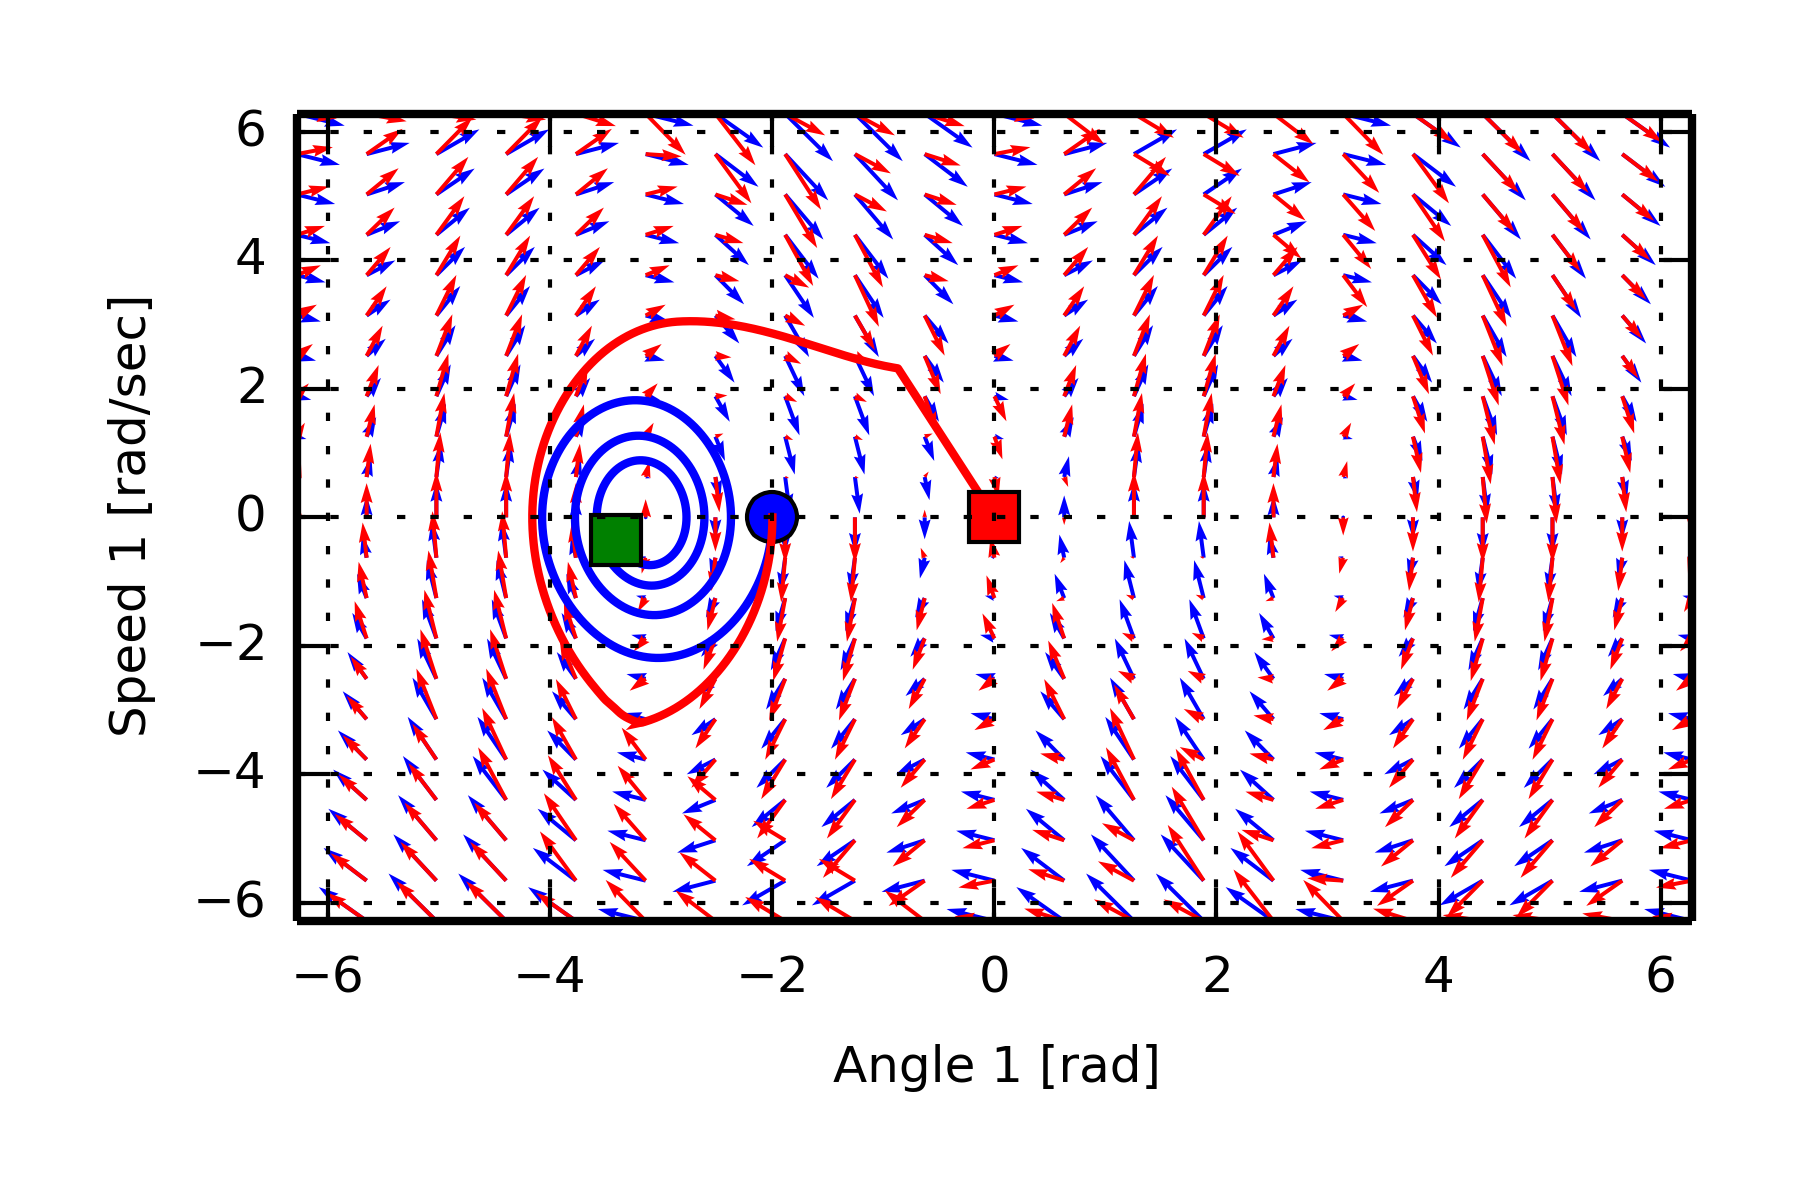
\includegraphics[width=0.48\textwidth]{PP_time.png}
				\label{fig:phase_plane_time}}
        \subfloat[Quadratic cost]{
				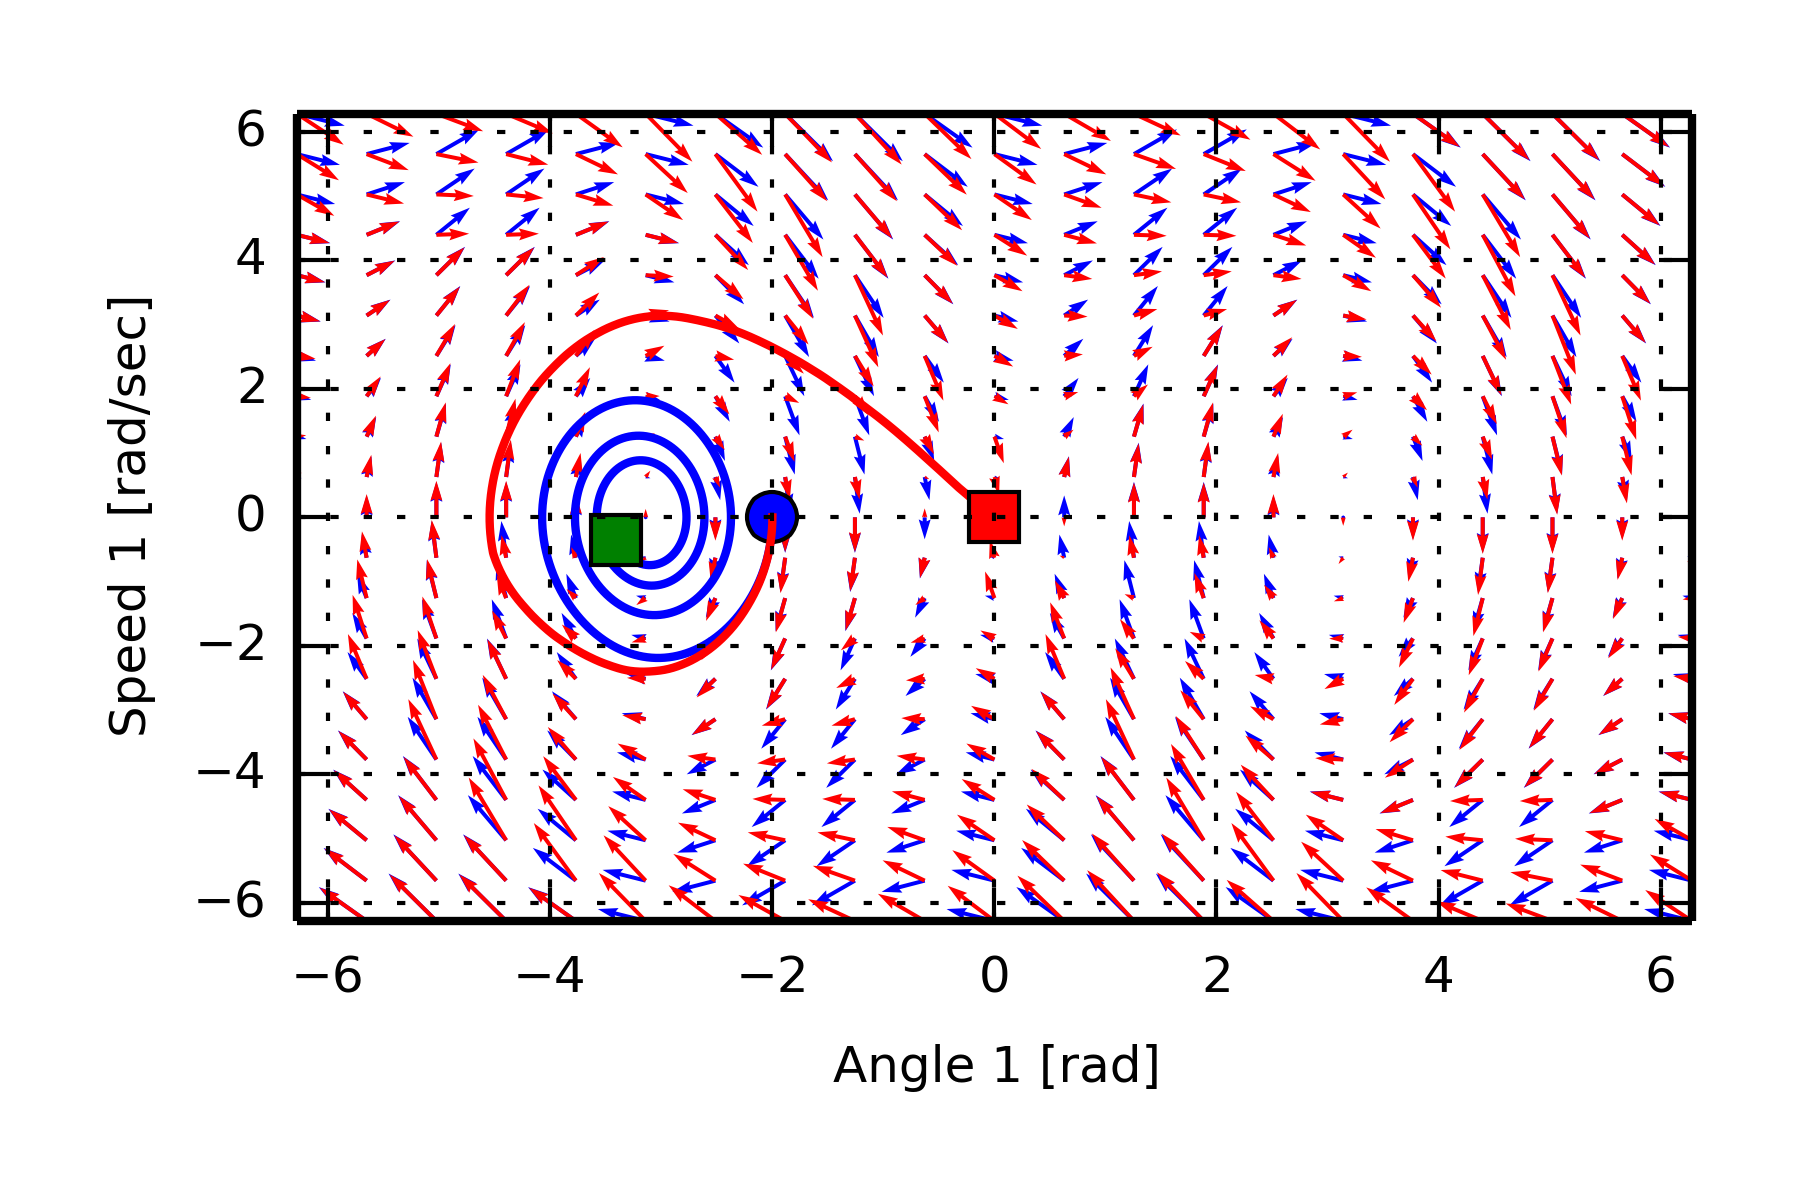
\includegraphics[width=0.48\textwidth]{PP_quadratic.png}
				\label{fig:phase_plane_LQR}}
        \caption[Closed loop behavior in the phase plane]{Closed loop behavior with the optimal policy illustrated in the phase plane. Two trajectories starting at $q=-2$ are illustrated, blue is open-loop, red is closed loop}\label{fig:phase_plane}
\end{figure*}


%\begin{figure*}[htpb]
        %\centering
				%\subfloat[Minimum time]{
        %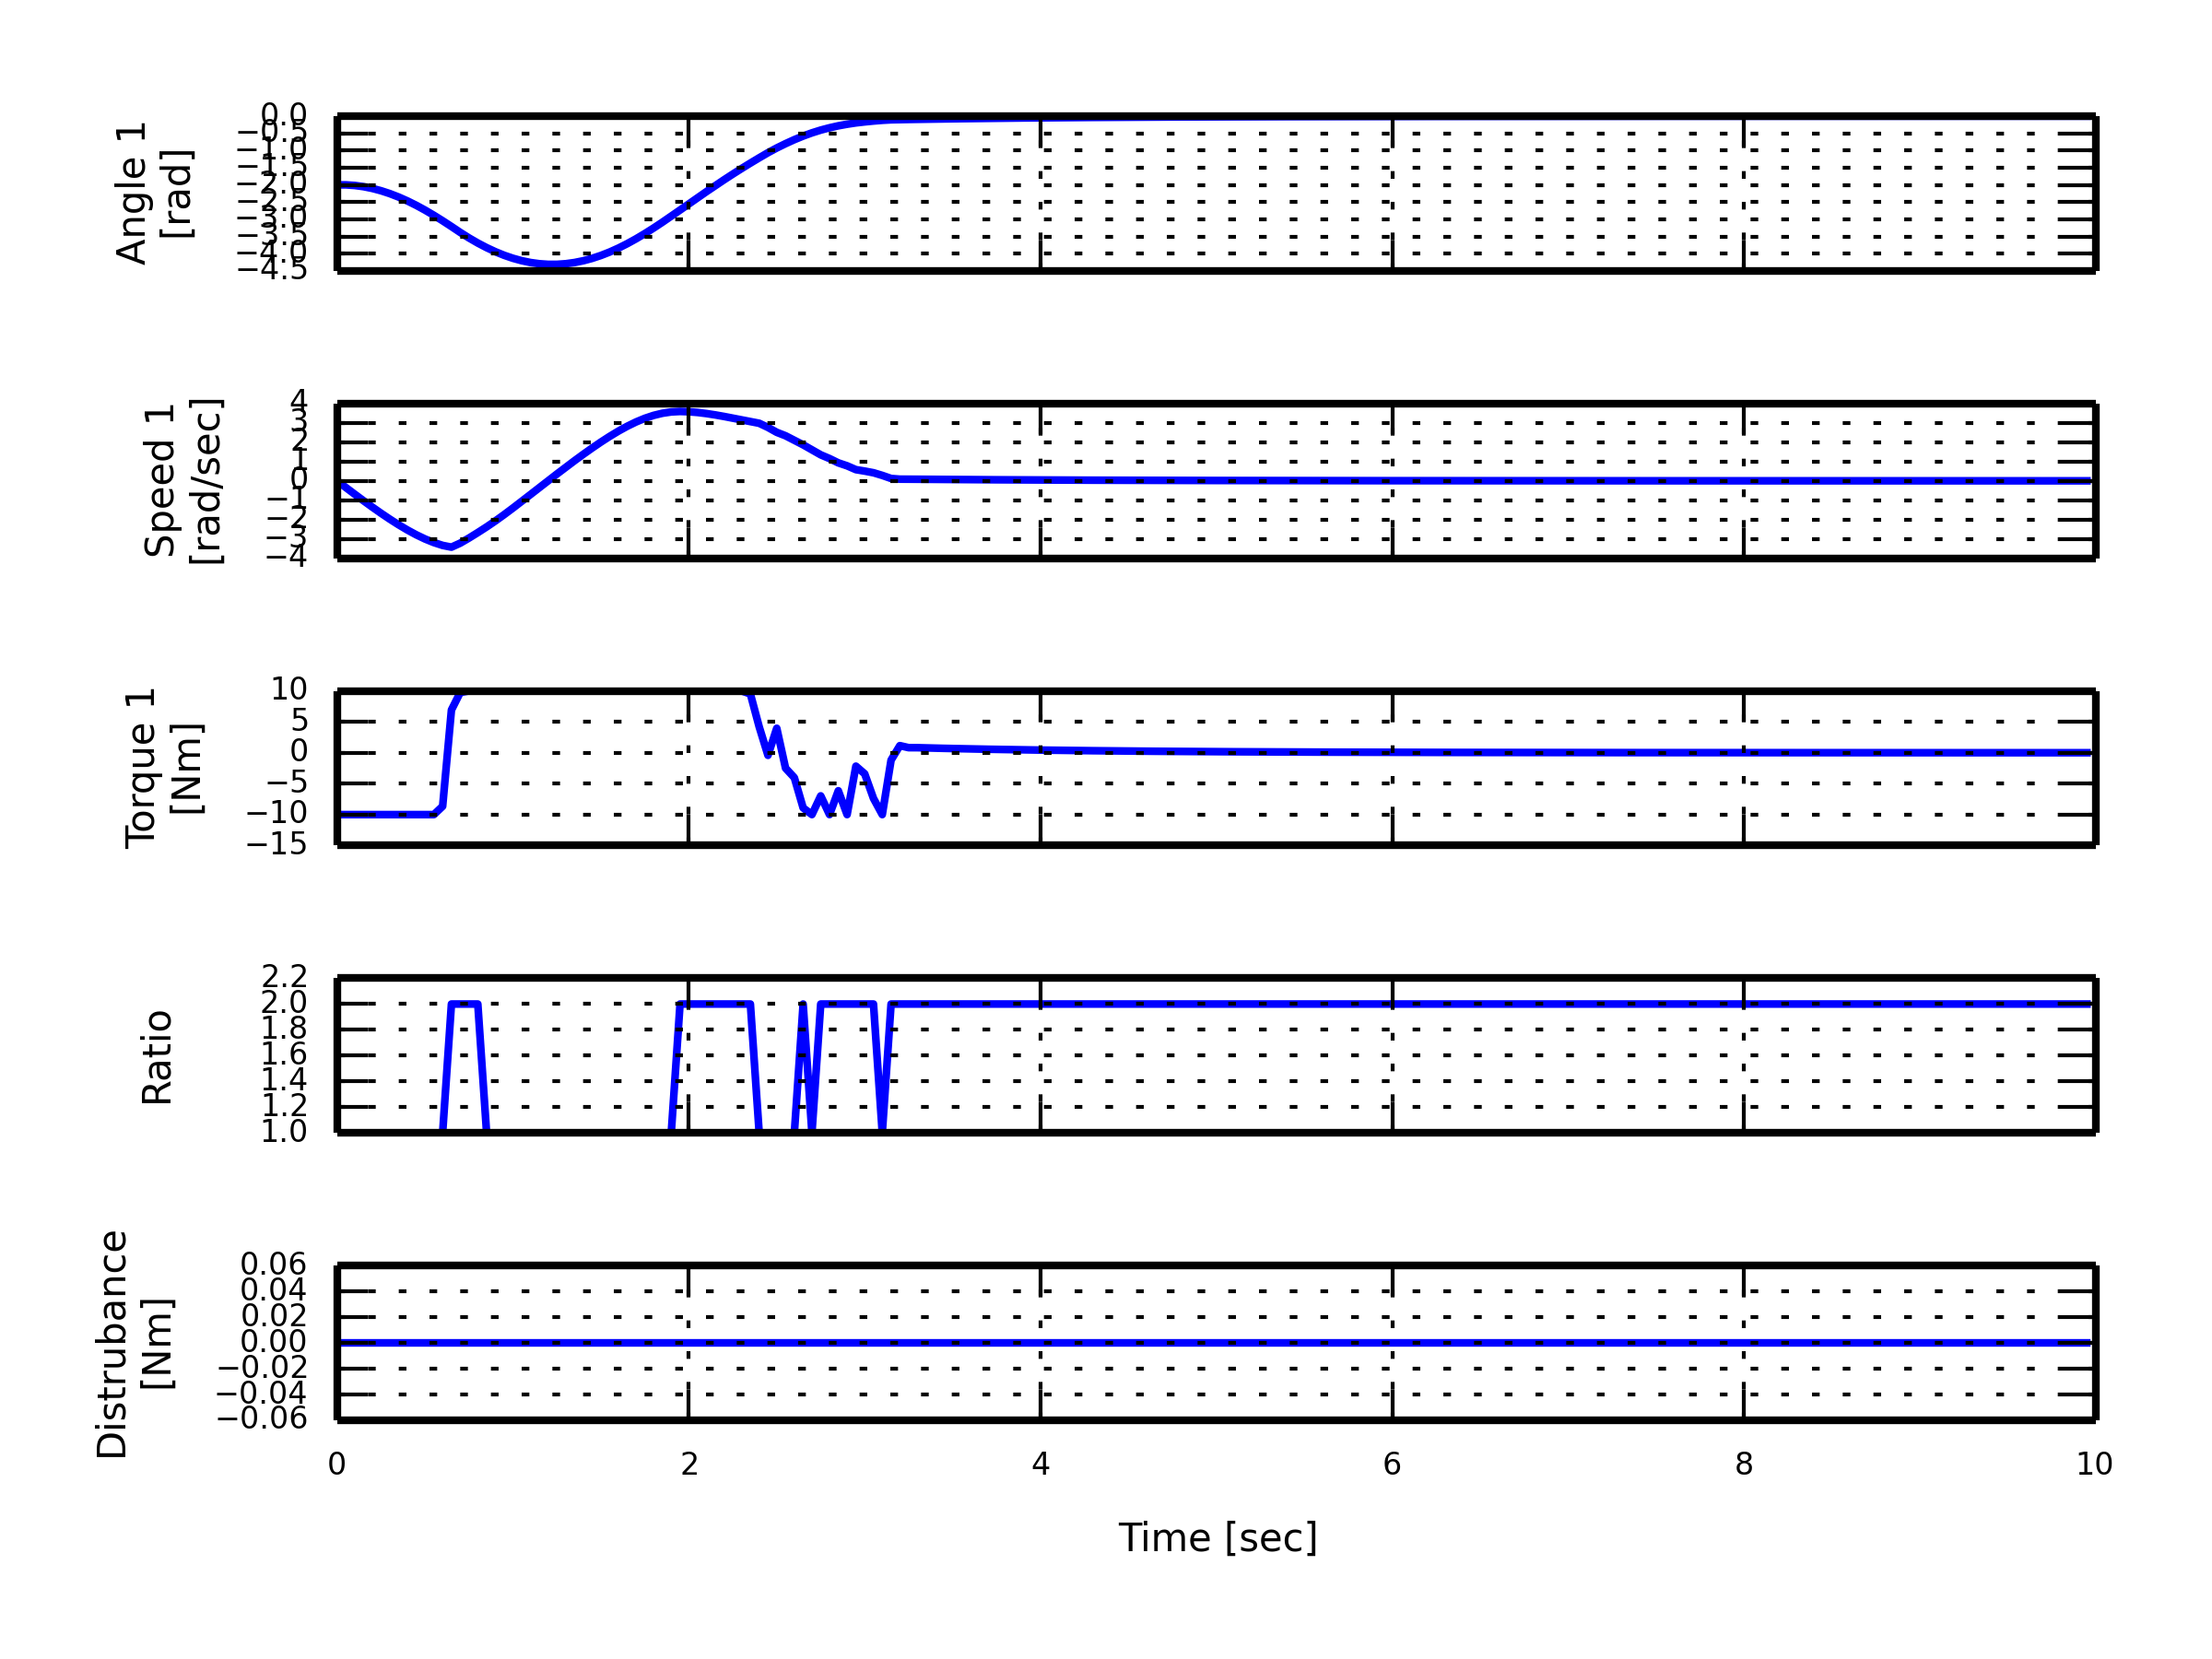
\includegraphics[width=0.48\textwidth]{Traj_time.png}
				%\label{fig:phase_plane_time}}
        %\subfloat[Quadratic cost]{
				%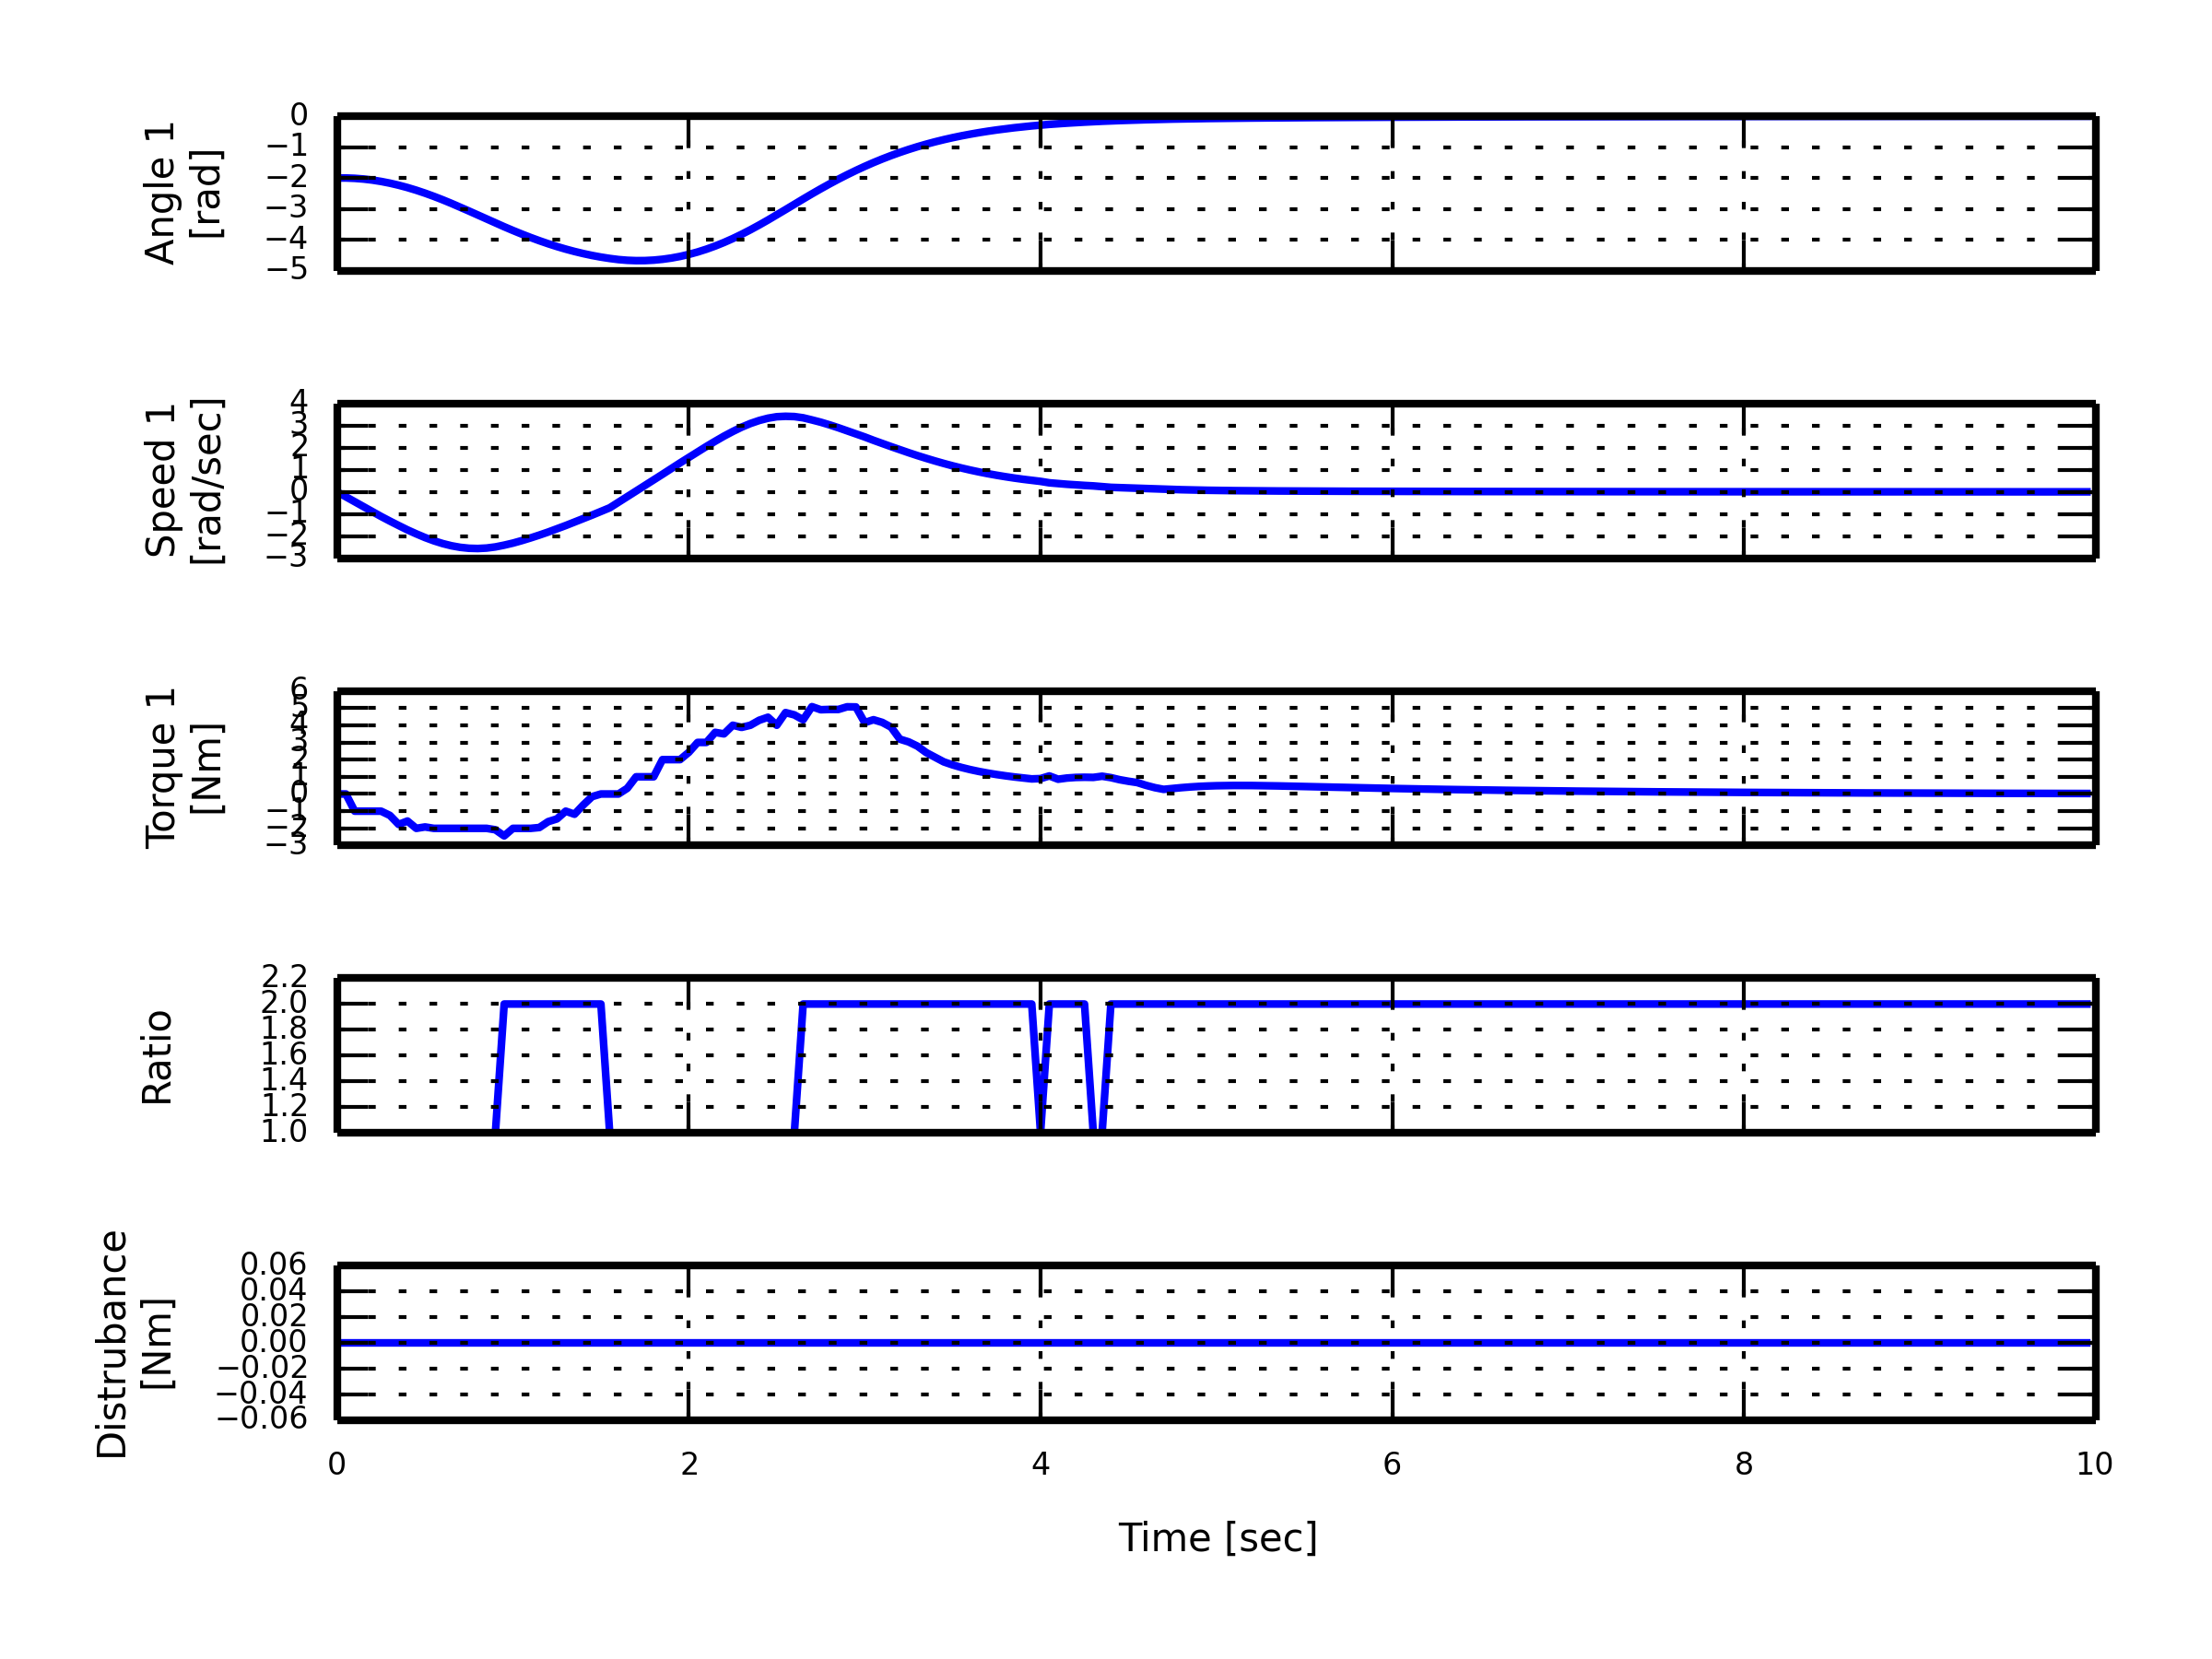
\includegraphics[width=0.48\textwidth]{Traj_quadratic.png}
				%\label{fig:phase_plane_LQR}}
        %\caption{State trajectories and control inputs for a closed loop simulation starting at $q=-2$}\label{fig:phase_plane}
%\end{figure*}

%The only issues that was found with those computations is that care need to be be used when picking the out-of bound termination conditions. Indeed, because of the stochastic state evolution, the high-cost assigned to out-of-bound terminations diffuse inside the boundary and reach states that should be able to never go out-of-bound (with a deterministic evolution). To alleviate this problem, the out-of-bound termination cost is set to a value just slightly bigger that the maximum expected optimal cost-to-go reaching the goal. Also, the boundary is set so that the boundary layer affected by this diffusion is not reaching the zone of interest.


%\subsection{Feedback laws simplification}
%
%TODO Using regresstion to obtain analytical feedback laws...
%
%In this section, simplified algebraic control laws are extracted from the numerical map of optimal control actions for the quadratic cost controller. The dynamic programming algorithm outputs a list of optimal actions that is assumed are samples of a  map of optimal actions $\vec{u}^* = \pi^* ( \vec{x} )$. The goal is then to find a simplified map $\hat{\pi}( \vec{x} )$ based on the samples. Here a two-steps approach is used; first the state-space is segmented into zones based on the optimal discrete action $u_2$, then regression is used to compute the $u_1$ map independently in each zone. 
%
%\subsubsection{1-DoF linear robot example}
%
%\paragraph{Segmentation}
%For the resulting optimal policy found at Fig. \ref{fig:u0_LQR}, three main zones can be identified. The boundaries are approximated by two lines at $\dot{x}= \pm \; 20 $, and the samples are separated into two groups:
%\begin{align}
%\left \{ \vec{u}^i , \vec{x}^i \right \} \rightarrow \text{Group 1} \quad \text{if} \; | \dot{x} | \geq 20 \\
%\left \{ \vec{u}^i , \vec{x}^i \right \} \rightarrow \text{Group 2} \quad \text{if} \; | \dot{x} | < 20
%\end{align}
%
%For more complex segmentation, machine learning techniques could be used to perform the classification.
%
%\paragraph{Continuous maps}
%
%In each zones, the optimal continuous input $u_1^*$ is very close to a planar surface with exceptions when the input saturates or near the boundaries, see Fig. \ref{fig:u0_LQR}. Here, it is proposed to forgo absolute optimality and instead use the simplest control law that can globally approximate $u_1^*$ map. Hence, simple linear plane are fitted on the samples group by group. The regression is defined as follow, the dependent variable to approximate is $u_1$, the independent variables are the state coordinates $\vec{x}^T = [ x  \; \dot{x} ]$ and the parameter vector is $\vec{\alpha}^T = [ k_p  \; k_d ]$. Hence the continuous control variable $\hat{u}_1$ is approximated with the following linear map:
%\begin{align}
%\hat{u}_1 = \vec{\alpha}^T \vec{x} = k_p  x + k_d \dot{x}
%\end{align}
%which is essentially a simple proportional-derivative control law. Then the parameters are estimated using a least-square criterion, $\vec{\alpha}_1$ using the samples in group 1 and $\vec{\alpha}_2$ samples in group 2. Then combining the segmentation and both linear maps, the global control policy is approximated with the following law:
%\begin{align}
%\vec{ \hat{u}} &= \hat{\pi} ( \vec{x} )
 %= \left \{ 
	%\begin{array}{c}
	%\left[
	%\begin{array}{c}
		 %\vec{\alpha}_1^T \vec{x} \\
		 %1 
	%\end{array} 
	%\right] 		
	%\text{if} \; | \dot{x} | \geq 20 \\ \\
		 %\left[
		%\begin{array}{c}
		 %\vec{\alpha}_2^T \vec{x} \\ 
		 %2
	%\end{array}
		 %\right]
		%\text{if} \; | \dot{x} | < 20
	%\end{array}
	%\right.
	%\label{eq:uhat}
%\end{align}
%Fig. \ref{fig:u0_LQR_approx} shows the resulting continuous control policy $\hat{u}_1$ for the full state-space, and is an approximation of Fig. \ref{fig:u0_LQR} map.
%
%%\begin{figure}[H]
	%%\centering
		%%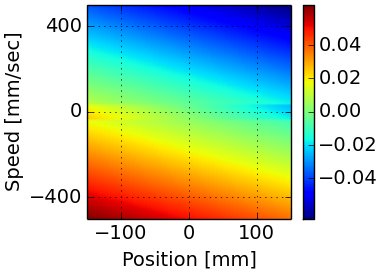
\includegraphics[width=0.30\textwidth]{u1aq.png}
	%%\caption{Continuous map approximation for $u_1$}
	%%\label{fig:u0_LQR_approx}
%%\end{figure}
%
%\begin{figure}[htpb]
				%\vspace{-10pt}
        %\centering
				%\subfloat[Map for $u_1$ (Nm)]{
        %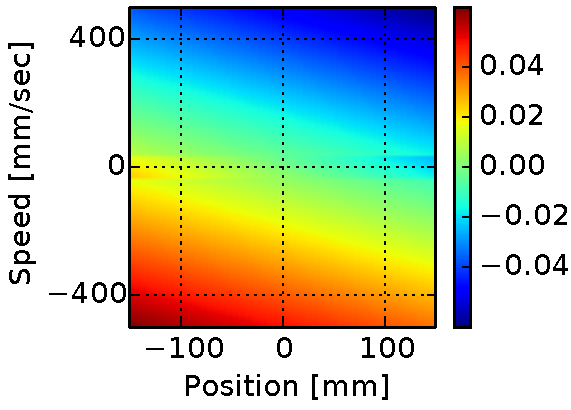
\includegraphics[width=0.45\textwidth]{u1aq.pdf}
				%\label{fig:u0_LQR_approx}}
        %\subfloat[Phase plane behavior]{
				%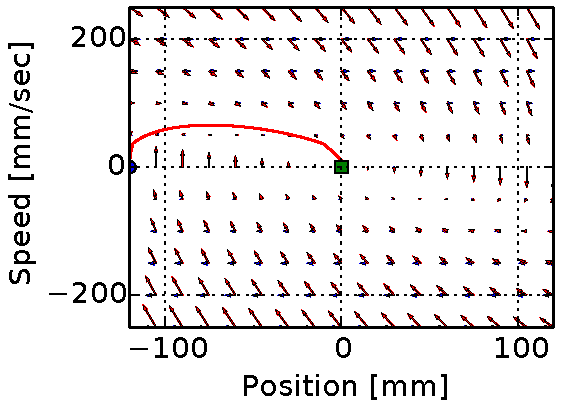
\includegraphics[width=0.40\textwidth]{pp2q.pdf}
				%\label{fig:phase_plot_lqr}}
        %\caption{Approximated control laws and resulting behavior}\label{fig:approx}
%\end{figure}
%
%
%The resulting behavior with the control law of eq.\eqref{eq:uhat} is illustrated in the phase plane at Fig. \ref{fig:phase_plot_lqr}, where the arrows illustrate the state derivative throughout the state space. The blue arrows illustrate the natural dynamic of the system and the red arrows illustrate the closed behavior with the control policy of eq.\eqref{eq:uhat}. At high speed with the small reduction ratio, the controller only takes small actions illustrated by the fact that red arrows only have small deviation compared to blue arrows. However at low speed, the large reduction ratio is used to drastically change the natural behavior of the system, illustrated by the large red arrows. 
%




%%%%%%%%%%%%%%%%%%%%%%%%%%%%%%%%%%%%%%%%%%%%%%%%%%%%%%%%%%%%%%%%%%%%%%%%%%%%%%%%%%%%%%%%%%%%%%%%%%%%%%%%%%%%%%%%%%%%%%%%%%%%%%%%%
\newpage
\section{Simulation Results}
\label{sec:shift_sim}


\subsection{Model-based controller}

In this section, the advantages of dynamically changing the gear-ratios, using the R* computed torque controller, are illustrated using simulations of two robots: first a 1-DoF pendulum, then a 3-DoF arm. Both robots are considered having VGA with two possible gear-ratios: 1:1 or 1:10. Reference low-torque trajectories to reach target positions are computed offline using a sample-based search algorithm \cite{lavalle_planning_2006}. 
%
The first simulated experiment uses the robot of Fig. \ref{fig:bigpicture}, but here considering dissipative forces in the actuators, with the task of reaching the up-right position starting at the bottom. Fig. \ref{fig:sim1} shows the robot tracking the reference low-torque trajectory, where at first the robot accumulates energy, using the 1:1 gear-ratio, and then finishes the motion using the 1:10 gear-ratio. When the gravitational forces are pushing advantageous toward the trajectory the controller select the 1:1 gear-ratio, but when it is advantageous to fight the intrinsic actuator dynamics instead, the 1:10 gear-ratio is selected. 

%
\begin{figure}[htp]
	\centering
		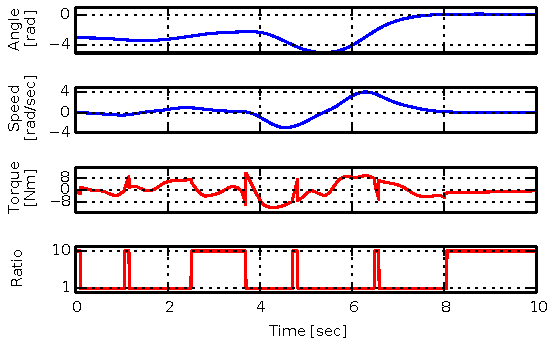
\includegraphics[width=0.75\textwidth]{sim1.pdf}
	\caption{1-DoF robot simulation: states and inputs trajectory}
	\label{fig:sim1}
\end{figure}
%
%
\begin{figure}[htp]
				\vspace{-10pt}
        \centering
				\subfloat[ Reduction ratio $R$=1 ]{ %extrinsic dynamics
				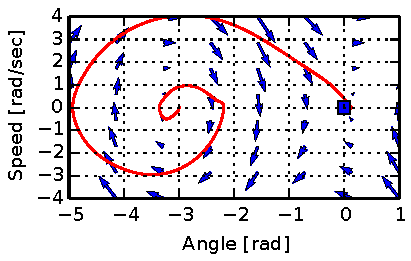
\includegraphics[width=0.45\textwidth]{simpp1.pdf}
				\label{fig:pp1s}}
        \subfloat[Reduction ratio $R$=10 ]{ % intrinsic dynamics
				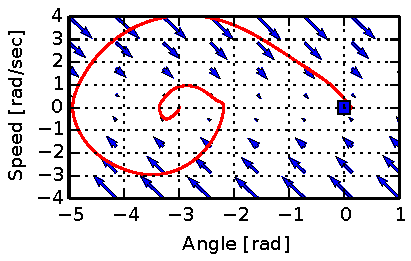
\includegraphics[width=0.45\textwidth]{simpp2.pdf}
				\label{fig:pp2s}}
        \caption{Trajectory superposed with natural dynamics vectors}
				\label{fig:pps}
\end{figure}

%\begin{figure}[htp]
	%\centering
		%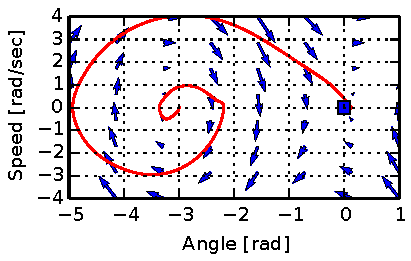
\includegraphics[width=0.38\textwidth]{simpp1.pdf}
	%\caption{Trajectory superposed with natural dynamics vectors with R=1}
	%\label{fig:simpp1}
%\end{figure}
%
%\begin{figure}[htp]
	%\centering
		%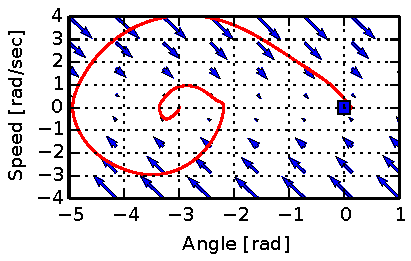
\includegraphics[width=0.38\textwidth]{simpp2.pdf}
	%\caption{Trajectory superposed with natural dynamics vectors with R=10}
	%\label{fig:simpp2}
%\end{figure}

In the second experiment, a 3-DoF manipulator is tasked with going from configuration A to configuration B with the 3D trajectory shown at Fig. \ref{fig:3d_traj}. For this robot the controller is actively selecting the best gear-ratios matrix $R$ out of the possible $2^3=8$ options. Fig. \ref{fig:3d_u} shows the control inputs activity. During the initial falling-down phase, at around $t=1$, the robot is using 1:1 gear-ratios for all actuators, leveraging gravitational torques. In contrast, during the final lifting phase, at around $t=6$, the robot is using 1:10 gear-ratios for all actuators. 
%
%
%
\begin{figure}[htp]
	\centering
		%\includegraphics[width=0.45\textwidth]{3dtraj.jpg}
		\includegraphics[width=0.75\textwidth]{3d_traj.pdf}
	\caption{ 3-DoF robot simulation: 3D trajectory }
	\label{fig:3d_traj}
\end{figure}
%
%\begin{figure}[htp]
	%\centering
		%\includegraphics[width=0.40\textwidth]{u_no4.pdf}
	%\caption{ 3-DoF robot simulation: control inputs trajectory where \textit{Mode} represent the index of the selected gear-ratio matrix }
	%\label{fig:3d_u}
%\end{figure}
%
\begin{figure}[htp]
	\centering
		\includegraphics[width=0.75\textwidth]{3d_u.pdf}
	\caption{ 3-DoF robot simulation: control inputs trajectory}
	\label{fig:3d_u}
\end{figure}
%%
%




\subsection{Value iteration}




\subsection{Comparison}


To evaluate the performance gain of actively changing the gear-ratio, simulations with fixed gear-ratios are conducted where a regular computed torque controller tracks the same trajectories. Results are summarized in TABLE \ref{tab:MaximumTorqueComparison}, in terms of maximum absolute torque, which relates to the required size and weight of motors, and integral of torque squared, which relates to power consumption. Active gear-ratio selection is found to greatly improve both metrics, especially for the 3-DoF robot trajectory where the arm must both achieve high-speeds and also sustain a constant gravitational load at the final configuration. Note that in those simulations high-velocity with 1:10 reductions is inhibited by friction in the motors, no maximum rotor velocity is enforced. For the 3-DoF trajectory, active gear-shifting is found to reduce the maximum torque required by a factor two and the integral of the torque square by a factor 10, compared to any of the fixed-gear options. Those results show the potential of using variable gear-ratio transmissions for huge improvements in terms of actuator size and power consumption. Moreover, here in the simulations, the load was always the same manipulator in different dynamic situations. As discussed in section \ref{sec:app}, if the load dynamics is radically changing because of different contact situations with the environment, the performance gain of changing the gear-ratio could be even greater. 
%
\begin{table}[htp]
	\centering
		\caption{Required torque comparison}
		\begin{tabular}{ c c c c }
		\hline
		     & Fixed gear & Fixed gear & Active gearshifting \\
			& 1:1 &  1:10 &  1:1 or 1:10 \\
		\hline \hline
		\multicolumn{4}{c}{ Max Absolute Torque [Nm] } \\
		\hline \hline
		1-link robot  & 15 & 88 & 12 \\	
		3-link robot  & 24 & 42 & 12 \\	
		\hline \hline
		\multicolumn{4}{c}{ Torque squared integral $\int{ ( \vec{\tau}^T \vec{\tau} ) dt }$ } \\
		\hline \hline
		1-link robot  & 377  & 8133 & 226  \\	
		3-link robot  & 2774 & 3617 & 295  \\	
		\hline \hline
		\end{tabular}
	\label{tab:MaximumTorqueComparison}
\end{table}
%



%%%%%%%%%%%%%%%%%%%%%%%%%%%%%%%%%%%%%%%%%%%%%%%%%%%%%%%%%%%%%%%%%%%%%%%%%%%%%%%%%%%%%%%%%%%%%%%%%%%%%%%%%%%%%%%%%%%%%%%%%%%%%%%%%


\section{Experiments Results}
\label{sec:shift_exp}

\subsection{Model-based controller}

First a trajectory following experiments using the last DoF of the robot only is presented. A 1.5 Kg load is mounted on the end-effector, and the task is to bring it from the bottom position ($q=-\pi$) to the up-right position ($q=0$) using as little torques as possible. An RRT trajectory planning algorithm is used to search for a low torque trajectory reaching the goal, see Fig. \ref{fig:exp_rrt}. Then the R* Computed Torque Controller is used to track the reference trajectory. The experimental results are shown in Fig. \ref{fig:exp_traj} and a video of this experiment is also available in the multimedia attachment. 
%
\begin{figure}[htp]
	\centering
		\includegraphics[width=0.75\textwidth]{rrt_fig.pdf}
	\caption{Trajectory generation algorithm searching for a low torque solution}
	\label{fig:exp_rrt}
\end{figure}
%
\begin{figure}[htp]
	\centering
		\includegraphics[width=0.75\textwidth]{exp_fig3.pdf}
	\caption{Experimental results}
	\label{fig:exp_traj}
	\vspace{-10pt}
\end{figure}
%
Results show that the robot is using its 1:23 gear-ratio to accumulate kinetic energy by swinging the arm link back and forth. Also the R* controller selects the 1:474 gear-ratio automatically to attenuate the load dynamics, when the actuator has to force the robot to stay with the trajectory.  Interestingly, the reference trajectory was planned so the robot would accumulate enough kinetic energy to swing straight up with the last swing. However, in the experiment, the dissipative forces are greater than anticipated by the planner, and the last swing is too small (the robot almost stop at $q=-0.9$ at $t=2.6$ in Fig. \ref{fig:exp_traj}). Then, the R* controller automatically engage the large 1:474 gear-ratio, to continue converging on the desired trajectory with much smaller torques than those required if keeping using the 1:23 gear-ratio in this situation (no momentum and a large gravitational force to overpower). This illustrates that including the gear-ratio selection in the feedback loop also increase the robustness of the system. Without the 1:474 gear-ratio option, tracking would have failed as the computed torque with 1:23 in this situation was greater than the maximum allowable motor torque.

Fig. \ref{fig:rob} shows four additional experiments for demonstrating how disturbance rejection can be improved by using the sliding mode version of the R* controller. Here the controller is only given a simple fixed point-target in all cases. First, when a low uncertainty bound is given to the controller, the robot can reach its target when unloaded (a) but failed when an unknown (to the controller) 0.4 Kg load is added to the end-effector (b). However, when a larger uncertainty bound is given, the robot can reach its target in both cases, unloaded (c) and loaded (d). Note that the discontinuous torque required to guarantee convergence despite disturbances is greatly reduced when down-shifting to a large gear-ratio at low speeds. For an improved performance, smoothing techniques should be implemented to avoid exciting the unmodeled high-frequency modes. Videos of all the experiments discussed above, and additional demonstrations are available in the media attachment.

\begin{figure}[htp]
				%\vspace{-10pt}
        \centering
				\hspace{-10pt}
				\subfloat[]{ % intrinsic dynamics
				\includegraphics[width=0.30\textwidth]{fig16a.pdf} }
				\hspace{-5pt}
        \subfloat[]{ % intrinsic dynamics
				\includegraphics[width=0.20\textwidth]{fig16b.pdf} }
				\hspace{-5pt}
				\subfloat[]{ % intrinsic dynamics
				\includegraphics[width=0.20\textwidth]{fig16c.pdf} }
				\hspace{-5pt}
				\subfloat[]{ % intrinsic dynamics
				\includegraphics[width=0.20\textwidth]{fig16d.pdf} }
        \caption{Experiments with sliding mode version of the R* controller }
				\label{fig:rob}
\end{figure}
